\documentclass[11pt]{book}
\usepackage{amsmath, amsthm, amssymb, bm, bbm}
\usepackage{amsfonts}
\usepackage{tikz}
\usepackage[utf8]{inputenc}
\usepackage[T1]{fontenc}
\usepackage{lmodern}

\usepackage{framed}
\definecolor{timberwolf}{rgb}{0.94, 0.94, 0.94}
\definecolor{azure}{rgb}{0.9, 0.95, 1.0}
\colorlet{shadedef}{timberwolf}
\colorlet{framedef}{timberwolf}
\colorlet{shadethm}{azure}
\colorlet{framethm}{azure}

\addtolength{\topmargin}{-1in}
\addtolength{\textwidth}{1in}
\addtolength{\evensidemargin}{-0.7in}
\addtolength{\textheight}{1.25in}

\newcommand{\norm}[1]{\left\lVert#1\right\rVert}
\newcommand{\inp}[2]{\langle #1,#2\rangle}
\newcommand{\vc}[1]{\textbf{\underline{#1}}}
\newcommand{\Ex}[0]{\vc{Ex}: }
\newcommand{\R}[1]{\mathbb{R}^{#1}}
\newcommand{\C}[1]{\mathbb{C}^{#1}}
\newcommand{\pf}[1]{\textbf{\underline{Proof}}: #1 $\;\;\blacksquare$}
\newcommand{\ub}[1]{\textbf{\underline{#1}}}
\newcommand{\OO}[0]{\mathcal{O}}
\newcommand{\TT}[0]{\mathcal{T}}
\newcommand{\CC}[0]{\mathcal{C}}
\newcommand{\FF}[0]{\mathcal{F}}
\newcommand{\MM}[0]{\mathcal{M}}
\newcommand{\HH}[0]{\mathcal{H}}
\newcommand{\Sm}[0]{\mathcal{S}}
\newcommand{\se}[0]{\subseteq}
\newcommand{\bint}[0]{\displaystyle\int}
\newcommand{\sif}[0]{\text{SIF}(S,\mu)}
\newcommand{\xsm}[0]{(X,\Sm,\mu)}


\newenvironment{prop}{%
  \def\FrameCommand{\fboxrule=\FrameRule\fboxsep=\FrameSep \fcolorbox{framethm}{shadethm}}%
  \MakeFramed {\FrameRestore}\noindent\textbf{\underline{Proposition}}:}%
{\endMakeFramed}

\newenvironment{lemma}{%
  \def\FrameCommand{\fboxrule=\FrameRule\fboxsep=\FrameSep \fcolorbox{framethm}{shadethm}}%
  \MakeFramed {\FrameRestore}\noindent\textbf{\underline{Lemma}}:}%
{\endMakeFramed}

\newenvironment{thm}{%
  \def\FrameCommand{\fboxrule=\FrameRule\fboxsep=\FrameSep \fcolorbox{framethm}{shadethm}}%
  \MakeFramed {\FrameRestore}\noindent\textbf{\underline{Theorem}}:}%
{\endMakeFramed}

\newenvironment{cor}{%
  \def\FrameCommand{\fboxrule=\FrameRule\fboxsep=\FrameSep \fcolorbox{framethm}{shadethm}}%
  \MakeFramed {\FrameRestore}\noindent\textbf{\underline{Corollary}}:}%
{\endMakeFramed}

\newenvironment{defn}{%
  \def\FrameCommand{\fboxrule=\FrameRule\fboxsep=\FrameSep \fcolorbox{framedef}{shadedef}}%
  \MakeFramed {\FrameRestore}\noindent\textbf{\underline{Def}}:}%
{\endMakeFramed}

\newenvironment{frame*}{%
  \def\FrameCommand{\fboxrule=\FrameRule\fboxsep=\FrameSep \fcolorbox{framethm}{shadethm}}%
  \MakeFramed {\FrameRestore}}%
{\endMakeFramed}


\title{Math 202A: Topology and Analysis I Lecture Notes}
\author{Joseph Pagadora \\ Instructor: Marc Rieffel}
\date{Fall 2018}

\begin{document}
\maketitle

\tableofcontents

\chapter{Metric Spaces}
\section{Fundamentals}
\begin{defn}
Let $X$ be a set. A \vc{metric} on $X$ is a function $d:X\times X\rightarrow [0,\infty)$ that satisfies: 
\begin{enumerate}
\item[(a)] $d(x,y)=d(y,x)$ for any $x,y\in X$
\item[(b)] $d(x,y)\leq d(x,z)+d(z,y)$ for any $x,y,z\in X$
\item[(c)] $d(x,y)=0$ iff $x=y$
\end{enumerate}
If a function $d$ satisfies (a), (b) above, and $d(x,x)=0$ for all $x\in X,$ then $d$ is a \vc{semi-metric}.
\end{defn}

\Ex On $\C{n},$ the following are common metrics:
\begin{itemize}
\item $d_p(v,w)=\Big(\sum\limits_{j=1}^n |v_j-w_j|^p\Big)^{1/p}$ for $p\geq 1$
\item $d_{\infty}(v,w)=\sup\{|v_j-w_j|:1\leq j\leq n\}$
\end{itemize}
(Verify that these are metrics.) \\ \\
Fact: If $S\subseteq X,$ and $d$ is a metric on $X,$ then $d$ is a metric on $S.$ \\

\begin{defn} 
Let $V$ be a vector space over $\R{ }$ or $\C{ }.$ A \vc{norm} on $V$ is a function $\norm{\cdot}:V\rightarrow[0,\infty)$ such that:
\begin{enumerate}
\item[(a)] $\norm{cv}=|c|\cdot\norm{v}$ for $c\in \R{}$ or $\C{}$ and $v\in V$
\item[(b)] $\norm{v+w}\leq\norm{v}+\norm{w}$ for $v,w\in V$
\item[(c)] $\norm{v}=0$ implies $v=0$
\end{enumerate}
A function that satisfies only (a) and (b) above is called a \vc{seminorm}.
\end{defn}

\noindent Remark: Any norm $\norm{\cdot}$ on $X$ induces the metric $d(x,y):=\norm{x-y}.$ \\ \\ \\
\Ex Let $V$ be the space of continuous functions on $[0,1].$ Then  \\ $\norm{f}_{\infty}=\sup\{|f(x)|:x\in[0,1]\}$ is a norm on $V.$ \\
It can also be shown that $\norm{f}_p:=\Big(\int_0^1 |f(x)|^p\;dx\Big)^{1/p}$ is a norm on $V.$ \\

\begin{defn}
Let $(X,d_x)$ and $(Y,d_y)$ be metric spaces. A function $f:X\rightarrow Y$ is \vc{isometric} if $d_y(f(v),f(w))=d_x(v,w)$ for all $v,w\in X.$
\end{defn}
\begin{itemize}
\item Note that all isometries are injective.
\end{itemize}

\noindent\Ex If $S\subseteq X,$ and $f:S\rightarrow X$ is defined by $f(x)=x$ (inclusion), then $f$ is an isometry. \\ \\
If $f$ is onto, then $f$ is viewed as an isomorphism between $(X,d_x)$ and $(Y,d_y).$ $f^{-1}$ is also an isomorphism.
\begin{defn} 
A function $f:X\rightarrow Y$ is \vc{Lipschitz} if there is a constant $k\geq 0$ such that $d_y(f(x_1),f(x_2))\leq k\cdot d_x(x_1,x_2).$ The smallest such constant is the \vc{Lipschitz constant} for $f.$
\end{defn}

\begin{defn} 
$f:X\rightarrow Y$ is \vc{uniformly continuous} if for any $\epsilon>0,$ there exists $\delta>0$ such that $d_y(f(x_1),f(x_2))<\epsilon$ whenever $d_x(x_1,x_2)<\delta.$
\end{defn}
\begin{itemize}
\item It is easy to see that if $f$ is Lipschitz, then it is uniformly continuous.
\end{itemize}

\begin{defn} 
$f:X\rightarrow Y$ is \vc{continuous at $x_0$} if for any $\epsilon>0,$ there exists $\delta>0$ such that $d_y(f(x),f(x_0))<\epsilon$ whenever $d_x(x,x_0)<\delta.$ We say $f$ is \vc{continuous} if it is continuous at every $x\in X.$
\end{defn}

\begin{defn} 
A sequence $\{x_n\}$ in $X$ \vc{converges} to $x^*\in X$ if for any $\epsilon>0,$ there exists $N\in\mathbb{N}$ such that for all $n\geq N,$ we have $d(x_n,x^*)<\epsilon.$
\end{defn}

\begin{prop} 
A function $f:X\rightarrow Y$ is continuous iff $x_n\rightarrow x$ implies $f(x_n)\rightarrow f(x).$ \\ \\
\pf{\textit{Exercise.}}
\end{prop}

\begin{defn}
$S\subseteq X$ is \vc{dense} in $X$ if for any $x\in X$ and $\epsilon>0,$ there exists $s\in S$ such that $d(x,s)<\epsilon.$
\end{defn}

\begin{prop}
Let $S$ be dense in $X,$ and let $f:X\rightarrow Y$ and $g:X\rightarrow Y$ be continuous functions such that $f(s)=g(s)$ for all $s\in S.$ Then $f=g$ on $X.$ \\ \\
\pf{Let $x\in X\setminus S,$ and let $\epsilon>0.$ Then there exists $\delta>0$ and $s\in S$ such that $d(f(x),f(s))<\epsilon/2,$ and $d(g(x),g(s))<\epsilon/2$ for $d(x,s)<\delta,$ by continuity and density. Then 
$$d(f(x),g(x))\leq d(f(x),f(s))+d(g(s),g(x))<\epsilon/2+\epsilon/2=\epsilon,$$
since $f(s)=g(s).$ Thus $d(f(x),g(x))=0,$ so $f(x)=g(x).$}
\end{prop}

\begin{defn}
A sequence $\{x_n\}$ is \vc{Cauchy} if for any $\epsilon>0,$ there exists $N\in\mathbb{N}$ such that $n,m\geq N$ implies $d(x_n,x_m)<\epsilon.$ \\
A metric space in which every Cauchy sequence converges is \vc{complete}.
\end{defn}

\noindent\Ex Consider $(\mathbb{Q}, |\cdot|).$ We know there exists a Cauchy sequence converging to $\sqrt{2}\in\mathbb{R},$ but in this metric space, $\sqrt{2}$ is not an element, so this sequence does not converge, hence this metric space is not complete.

\section{Completion of a Metric Space}

\begin{prop}
If $f:X\rightarrow Y$ is uniformly continuous, and $\{x_n\}$ is Cauchy in $X,$ then $\{f(x_n)\}$ is Cauchy in $Y.$ \\ \\
\pf{\textit{Exercise.}}
\end{prop}

\begin{defn}
Let $(X,d)$ be a metric space. A complete metric space $(\overline{X},\overline{d}),$ together with an isometric function $f:X\rightarrow\overline{X}$ with dense range is a \vc{completion} of $(X,d).$
\end{defn}
\begin{itemize}
\item Remark: Completions are unique up to isomorphism.
\end{itemize}

\begin{prop}
If $((Y_1, d_1), f_1)$ and $((Y_2,d_2),f_2)$ are completions of $(X,d),$ then there exists an onto isometry (metric space isomorphism) $g:Y_1\rightarrow Y_2$ with $f_2=g\circ f_1.$ This can be visualized by the following commutative diagram: \\
\begin{center}
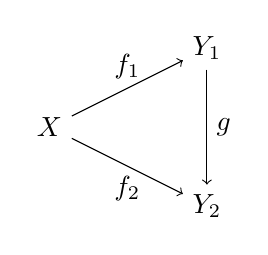
\begin{tikzpicture}
\node (a) at (0,0) {$X$};
\node (b) at (2,1) {$Y_1$};
\node (c) at (2,-1) {$Y_2$};
\draw[->] (a) -> (b) node[midway,above] {$f_1$};
\draw[->] (a) -> (c) node[midway,below] {$f_2$};
\draw[->] (b) -> (c) node[midway,right] {$g$};
\end{tikzpicture}
\end{center}
\end{prop}

\noindent Every metric space has a completion, and the proof will be constructive. The completion will be defined using equivalence classes of Cauchy sequences. We will need the following lemmas to support the construction.

\begin{frame*}
\noindent \ub{Lemma 1}: If $\{s_n\}$ and $\{t_n\}$ are Cauchy sequences in $X,$ then the sequence $\{d(s_n,t_n)\}$ in $\R{}$ converges. \\
\pf{\textit{Exercise. Hint:} $\{d(s_n,t_n)\}$ is a Cauchy sequence in a complete metric space.}
\end{frame*}

\begin{frame*}
\noindent \ub{Lemma 2}: Let $\text{Cau}(X)$ denote the set of all Cauchy sequences in $X.$ Then the relation $\{s_n\}\sim \{t_n\}$ iff $d(s_n,t_n)\rightarrow 0$ is an equivalence relation. \\ \\
\pf{Reflexivity and symmetry are trivial. Suppose $d(s_n,r_n)\rightarrow 0$ and $d(r_n,t_n)\rightarrow 0.$ Then $d(s_n,t_n)\leq d(s_n,r_n)+d(r_n,t_n)$ for all $n\in\mathbb{N}.$ The result follows immediately.}
\end{frame*}

\begin{frame*}
\noindent \ub{Lemma 3}: Let $\overline{X}$ be the set of all equivalence classes of $\text{Cau}(X)$ under the equivalence relation above. Then $\overline{d}:\overline{X}\rightarrow[0,\infty)$ defined by $\overline{d}(\{s_n\},\{t_n\}):=\lim\limits_{n\rightarrow\infty} d(s_n,t_n)$ is a metric on $\overline{X}.$ \\ \\
\pf{First, note that by Lemma 1, $\overline{d}$ is always defined. Since we are dealing with equivalence classes, we must show that $\overline{d}$ is also well-defined. Let $\xi,\eta\in\overline{X},$ and let $\{x_n\},\{s_n\}\in\xi,$ and $\{y_n\},\{t_n\}\in\eta.$ We have $\lim d(x_n,s_n)=\lim d(y_n,t_n)=0.$ Thus, \\ $d(s_n,t_n)\leq d(s_n,x_n)+d(x_n,y_n)+d(y_n,t_n).$ For any $\epsilon>0,$ we can find $N\in\mathbb{N}$ such that both $d(s_n,x_n)<\epsilon/2$ and $d(y_n,t_n)<\epsilon/2$ for $n\geq N.$ Then $|d(s_n,t_n)-d(x_n,y_n)|<\epsilon.$ It follows that $\overline{d}(\xi,\eta)=\lim d(x_n,y_n)=\lim d(s_n, t_n),$ so that $\overline{d}$ is indeed well-defined. \\  \\
Symmetry is trivial. The triangle inequality follows from the proof to Lemma 2. If $\overline{d}(\xi,\eta)=0,$ then for any $\{x_n\}\in\xi, \{y_n\}\in\eta,$ we have $\lim d(x_n,y_n)=0,$ so in particular, $\{y_n\}\in\xi,$ hence $\xi=\eta.$}
\end{frame*}

\begin{thm}
Let $(X,d_x)$ and $(Y,d_y)$ be metric spaces with $Y$ complete. If $S\subseteq X$ is dense, and $f:S\rightarrow Y$ is uniformly continuous, then there exists a unique continuous extension $\overline{f}:X\rightarrow Y$ of $f.$ In fact, $\overline{f}$ is uniformly continuous. \\ \\
\pf{(Existence only) For $x\in X,$ choose a Cauchy sequence $\{s_n\}$ in $S$ converging to $x.$ Then $\{f(s_n)\}$ is Cauchy in $Y,$ so it converges to a point $p\in Y.$ Set $\overline{f}(x):=p.$ We show that $\overline{f}$ is well-defined. Indeed, if $\{t_n\}\in\text{Cau}(S)$ and converges to $x,$ then we have $\lim d_x(s_n,t_n)=0,$ implying that $\lim d_y(f(s_n),f(t_n))=0.$ Therefore $\lim d_y(f(t_n),p)=0,$ so $\{f(t_n)\}$ converges to $p$ also. It remains to show continuity, which is left as an exercise.}
\end{thm}

\begin{thm}
Every metric space $(X,d)$ has a completion. \\ \\
\pf{As in Lemma 3, $(\overline{X},\overline{d})$ is a completion of $(X,d).$ We embed $X$ in $\overline{X}$ by the isometry $\iota:X\rightarrow\overline{X}$ defined by $\iota(x):= [\{x,x,x,...\}],$ where $[\cdot]$ denotes the corresponding equivalence class. Note that $\overline{d}\Big|_X=d,$ i.e., $\overline{d}(\iota(x),\iota(y))=d(x,y).$\\ It remains to show that $\overline{d}$ has dense range, and that $(\overline{X},\overline{d})$ is complete.
\begin{itemize}
\item Let $\xi\in\overline{X}, \epsilon>0, \{x_n\}\in\xi.$ There exists $N\in\mathbb{N}$ such that $n,m\geq N$ implies $d(x_n,x_m)<\epsilon.$ Then $\overline{d}(\iota(x_N),\xi)=\lim\limits_{n\rightarrow\infty} d(x_N,x_n)<\epsilon.$ Therefore $\overline{d}$ has dense range by considering $\iota(x_N).$
\item Let $\{\xi_n\}$ be a Cauchy sequence in $\overline{X}.$ For each $m\in\mathbb{N},$ pick $x_m\in X$ such that $\overline{d}(\iota(x_m),\xi_m)<1/m.$ Then $\{x_m\}$ is a Cauchy sequence, and it follows that $\{\xi_m\}$ converges to the equivalence class of $\{x_m\}.$
\end{itemize}}
\end{thm}

\noindent Remark on functions:\\
Denote $C([0,1])$ the space of continuous functions on $[0,1].$ Consider the metric space $C([0,1])$ induced by the norms $\norm{\cdot}_{\infty}$ or $\norm{\cdot}_p.$ This space is not complete. It is easy to come up with a sequence of continuous functions converging under these norms to a function that is not continuous. \\

\noindent Vector Space Remark: \\
Let $V$ be a vector space with norm $\norm{\cdot}.$ Consider $V^{\infty},$ the space of all sequences of elements in $V.$ This is also a vector space. It can be shown that $\text{Cau}(V)$ is a subspace of $V^{\infty}.$ \\
Now let $\mathcal{N}(V)$ denote the set of all Cauchy sequences in $V$ converging to $0.$ Then $\mathcal{N}(V)$ is a subspace of $\text{Cau}(V).$ If $\{v_n\}$ and $\{w_n\}$ are equivalent Cauchy sequences, then \\ $\norm{v_n-w_m}\rightarrow 0,$ so $\{v_n-w_n\}\in\mathcal{N}(V).$ Thus $\overline{V}$ is in fact the quotient space $\text{Cau}(V)/\mathcal{N}(V).$ \\ \\
Fact: Any two norms $\norm{\cdot}_1,\norm{\cdot}_2$ on a finite dimensional vector space are \ub{equivalent}, meaning that there are constants $c,C>0$ such that $c\norm{x}_1\leq\norm{x}_2\leq C\norm{x}_1$ for all $x.$ If a function is continuous with respect to a particular norm, then it is easily seen that it is continuous with respect to any equivalent norm.

\section{Openness}

\begin{defn}
If $(X,d)$ is a metric space, the \ub{open ball} of radius $r$ around $x$ is \\ $B_r(x):=\{y\in X: d(x,y)<r\}.$
\end{defn}

\begin{defn}
We can rephrase continuity as $f:X\rightarrow Y$ is continuous at $x_0$ if for any $\epsilon>0,$ there exists $\delta>0$ such that $f\Big(B_{\delta}(x_0)\Big)\subseteq B_{\epsilon}(f(x_0)).$
\end{defn}

\noindent
If $y\in B_{\epsilon}(f(x_0))$ and $y=f(x)$ for some $x\in X,$ let $\epsilon'=\epsilon-d(y,f(x_0))>0.$ Then $B_{\epsilon'}(y)\subseteq B_{\epsilon}(f(x_0)),$ so there exists $\delta'>0$ such that $f\Big(B_{\delta'}(x)\Big)\subseteq B_{\epsilon}(f(x_0)).$ \\
If $x_1\in f^{-1}\Big(B_{\epsilon}(f(x))\Big),$ there is an open ball $B_{\delta'}(x)$ such that $B_{\delta'}(x_1)\subseteq f^{-1}\Big(B_{\epsilon}(f(x))\Big).$ Thus $f^{-1}\Big(B_{\epsilon}(f(x))\Big)$ is a union of open balls in $X.$ Similarly, $f^{-1}(B_{\epsilon}(y))$ is a union of open balls in $X.$

\begin{defn}
A subset $\mathcal{O}\subseteq X$ (where $X$ is a metric space) is \ub{open} if it is a union of open balls in $X.$
\end{defn}

By the arguments above, it can be shown that $f:X\rightarrow Y$ is continuous iff for any open ball $B_{\epsilon}(y)\subseteq Y,$ we have that $f^{-1}(B_{\epsilon}(y))$ is open in $X.$ \\

\noindent Set theoretic facts:\\
Let $f:X\rightarrow Y$ be a function, and let $\{A_{\alpha}\}$ be a family of subsets of $X.$ Then:
\begin{itemize}
\item $f^{-1}\Big(\bigcup_{\alpha} A_{\alpha}\Big) = \bigcup_{\alpha} f^{-1}(A_{\alpha})$
\item $f^{-1}\Big(\bigcap_{\alpha} A_{\alpha}\Big) = \bigcap_{\alpha} f^{-1}(A_{\alpha})$
\item $f^{-1}\Big(A_1\setminus A_2) = f^{-1}(A_1)\setminus f^{-1}(A_2)$
\item $f\Big(\bigcup_{\alpha} A_{\alpha}\Big) = \bigcup_{\alpha} f(A_{\alpha})$
\item $f\Big(\bigcap_{\alpha} A_{\alpha}\Big) \subseteq \bigcap_{\alpha} f(A_{\alpha})$
\item $f(A_1\setminus A_2)\supseteq f(A_1)\setminus f(A_2)$
\end{itemize}

\noindent Let $\mathcal{O}\subseteq Y$ be open. Then $f^{-1}(\mathcal{O})=f^{-1}\Big(\bigcup\limits_{U\subseteq\mathcal{O}, U\text{ open ball}} U\Big)=\bigcup\limits_{U\subseteq\mathcal{O}, U\text{ open ball}} f^{-1}(U).$ \\ Thus, if $f:X\rightarrow Y$ is continuous, and $\mathcal{O}$ is open in $Y,$ then $f^{-1}(\mathcal{O})$ is open in $X.$
\begin{thm}
If $(X,d)$ is a metric space, and $\tau_d$ is the collection of all open sets, then:
\begin{enumerate}
\item[(1)] If $\{\mathcal{O}_{\alpha}\}$ is an arbitrary collection of subsets in $\tau_d,$ then $\bigcup_{\alpha}\mathcal{O}_{\alpha}$ is open.
\item[(2)] If $\mathcal{O}_1,\hdots,\mathcal{O}_n$ is a finite collection of subsets in $\tau_d,$ then $\bigcap\limits_{j=1}^n \mathcal{O}_j$ is open.
\item[(3)] $X\in\tau_d$ ($X$ is open)
\end{enumerate}
\pf{
  \begin{enumerate}
  \item[(1)] Trivial
  \item[(2)] Let $x\in \bigcap\limits_{j=1}^n \mathcal{O}_j.$ For each $j,$ there exists $\delta_j>0$ such that $B_{\delta_j}(x)\subseteq\mathcal{O}_j.$ Let \\ $\delta=\min\{\delta_j:1\leq j\leq n\}.$ Then $B_{\delta}(x)\subseteq\mathcal{O}_j$ for each $j.$ This yields the desired result.
  \item[(3)] Let $\epsilon>0.$ Then $X=\bigcup\limits_{x\in X} B_{\epsilon}(x).$ The result follows from (1).
  \end{enumerate}
}
\end{thm}
\noindent By convention, $\varnothing\in\tau_d$ ($\varnothing$ is open).

\chapter{Introduction to Topology}
\section{Fundamentals}
\begin{defn}
Let $X$ be a set. A \ub{topology} on $X$ is a collection $\TT\subseteq\mathcal{P}(X)$ that satisfies:
\begin{enumerate}
\item[(1)] For any arbitrary family $\{\OO_{\alpha}\}\subseteq\TT,$ we have $\bigcup\limits_{\alpha}\OO_{\alpha} \in\TT.$
\item[(2)] For $\OO_1,\hdots,\OO_n\in\TT,$ we have $\bigcap\limits_{j=1}^n \OO_j\in\TT.$
\item[(3)] $X\in\TT, \varnothing\in\TT.$
\end{enumerate}
\end{defn}

\begin{defn}
\begin{itemize}
\item If $\TT$ is a topology on $X,$ then $(X,\TT)$ is a \ub{topological space}. The sets in $\TT$ are called \ub{open}, and the complements of the sets in $\TT$ are \ub{closed}.
\item For any $A\subseteq X,$ there is a smallest closed set containing $A,$ namely, the intersection of all closed sets containing $A$ (by DeMorgan's Laws, the arbitrary intersection of closed sets is closed). We denote such a set by the \ub{closure} of $A,$ denoted $\overline{A}.$
\item If $\TT_1$ and $\TT_2$ are topologies on $X,$ and $\TT_1\subseteq\TT_2,$ we say that $\TT_1$ is \ub{weaker/coarser} than $\TT_2.$ $\TT_2$ is \ub{stronger/finer} than $\TT_1.$
\end{itemize}
\end{defn}

\begin{prop}
For any sets $A,B$ in a topological space, $\overline{A\cup B}=\overline{A}\cup\overline{B}.$ \\ \\
\pf{\textit{Exercise}.}
\end{prop}

\noindent Let $\CC$ be a collection of topologies on $X.$ It can be shown that $\bigcap\limits_{\TT\in\CC}\TT$ is a topology on $X.$ From this fact, it follows that for any non-empty collection $\mathcal{S}$ of subsets of $X,$ there is a smallest topology on $X$ that contains $\mathcal{S}.$

\begin{defn}
Let $\mathcal{B}\subseteq\TT.$ We say that $\mathcal{B}$ is a \ub{base} for $\TT$ if every element of $\TT$ is a union of elements in $\mathcal{B}.$
\end{defn}

\begin{prop}
Let $X$ be a set, and let $\mathcal{B}$ be a collection of subsets of $X.$ If $\mathcal{B}$ has the property that for any $U,V\in\mathcal{B},$ $U\cap V$ is a union of elements of $\mathcal{B},$ then the collection of unions of elements of $\mathcal{B},$ then the collection of unions of elements in $\mathcal{B}$ is a topology for which $\mathcal{B}$ is a base. \\ \\
\pf{\textit{Exercise}.}
\end{prop}

\begin{defn}
Let $\mathcal{S}$ be any collection of subsets of $X$ such that $\bigcup\limits_{V\in\mathcal{S}} V=X,$ and the set of finite intersections of elements of $\mathcal{S}$ is a base for a topology, then $\mathcal{S}$ is a \ub{sub-base} for that topology.
\end{defn}

\noindent \Ex The standard metric topology on $\R{n}$ has the base $\{B_r(x):r>0,\;x\in\R{n}\}.$ \\ A sub-base for $\R{}$ with the metric topology is the collection of open rays: $(-\infty,a)$ and $(b,\infty).$ \\
\Ex Given a metric space $(X,d),$ we will always assume that it has a standard topology whose base consists of the open balls: $\{B_r(x):r>0,\;x\in X\}.$

\section{Continuity}

\begin{defn}
Let $(X,\TT_x)$ and $(Y,\TT_y)$ be topological spaces. A function $f:X\rightarrow Y$ is \ub{continuous} for $\TT_x$ and $\TT_y$ if for any $U\in\TT_y,$ we have $f^{-1}(U)\in\TT_x.$
\end{defn}

\noindent\begin{itemize}
\item It is clear that any composition of continuous functions on topological spaces is continuous.
\item For any topological space $(X,\TT),$ the identity map $\iota:X\rightarrow X$ is continuous.
\item The collection of topological spaces with continuous functions between them is a category.
\end{itemize}

\begin{defn}
$f:X\rightarrow Y$ is \ub{homeomorphic} if $f$ is continuous, bijective, and has a continuous inverse.
\end{defn}

\begin{prop}
$f:(X,\TT_x)\rightarrow (Y,\TT_y)$ is continuous iff for a base or sub-base $\CC$ for $\TT_y,$ we have $f^{-1}(U)\in\TT_x$ for $U\in\CC.$ \\ \\
\pf{The forward direction is obvious. For the converse, we prove the case for $\CC$ a base. The case for $\CC$ a sub-base follows similarly (add on finite intersections). \\ Suppose $f^{-1}(U)\in\TT_x$ for any $U\in\CC.$ Let $V\in\TT_y.$ Since $\CC$ is a base, there is a collection of open sets $\mathcal{B}\subseteq\CC$ such that $V=\bigcup\limits_{A\in\mathcal{B}} A.$ Then $f^{-1}(V)=f^{-1}\Big(\bigcup\limits_{A\in\mathcal{B}} A\Big)=\bigcup\limits_{A\in\mathcal{B}} f^{-1}(A)\in\TT_x,$ since each $f^{-1}(A)$ is open.}
\end{prop}

\noindent\begin{itemize}
\item Let $X$ be a set and let $(Y_{\alpha},\TT_{\alpha})$ be a collection of topological spaces, and for each $\alpha,$ let $f_{\alpha}:X\rightarrow Y_{\alpha}$ be a function. Then there is a smallest topology on $X$ for which each $f_{\alpha}$ is continuous, namely, the smallest topology having as sub-base all sets $f^{-1}_{\alpha}(U),$ where $U\in\TT_{\alpha}$ for all $\alpha.$
\item Let $(X,\TT_x)$ be a topological space, and let $Y$ be a set with $f:X\rightarrow Y$ a function. What is the strongest topology on $Y$ making $f$ continuous?
\begin{itemize}
\item We need that if $A\subseteq Y$ is open, then $f^{-1}(A)\in\TT_x.$ \\ Let $\TT:=\{A\subseteq Y: f^{-1}(A)\in\TT_x\}.$ Then $\TT$ is easily seen to be a topology on $Y.$ This is called the \ub{quotient topology} on $Y$ for $f.$
\end{itemize}
\item Note that if $y\not\in f(X),$ then $f^{-1}(\{y\})=\varnothing,$ so $\{y\}$ is open. Also, $f^{-1}(\{y\}^c)=X,$ so $\{y\}$ is also closed. Therefore, on $f(X)^c,$ the quotient topology is discrete. Thus, we usually require $f:X\rightarrow Y$ to be onto.
\end{itemize}

\section{Quotient and Product Topologies}
Let $f:X\rightarrow Y$ be onto, and define the equivalence relation on $X$ by $x_1\sim x_2$ iff $f(x_1)=f(x_2).$ Conversely, given any set $X,$ and an equivalence relation on $X,$ let $Y$ be the set of equivalence classes for $\sim.$ We often denote $Y$ by $X/\sim.$ Thus, given a topology on $X,$ we get the \ub{quotient topology} on $X/\sim.$ \\ \\
Given a collection $\{(X_{\alpha},\TT_{\alpha})\}$ of topological spaces and a set $Y,$ and for each $\alpha$ a function $f_{\alpha}:X_{\alpha}\rightarrow Y,$ the strongest topology on $Y$ making all $f_{\alpha}$ continuous is the intersection of all quotient topologies for each $f_{\alpha}.$ This is called the \ub{final topology}. \\ \\
\Ex Let $X=[0,1].$ Define the equivalence relation $s\sim t$ iff $s=t,$ and have $0\sim 1.$ That is, $\{0,1\}$ is an equivalence class.
\begin{center}
\begin{tikzpicture}
\node[circle, fill=black, inner sep=0pt, minimum size=0.5pt, scale = 1, label = left:{$0$}] (a) at (-4,0) {};
\node[circle, fill=black, inner sep=0pt, minimum size=0.5pt, scale = 1, label = right:{$1$}] (b) at (-2,0) {};
\draw[-] (a) -- (b) node[midway, above] {$X$};
\draw[fill=black] (-4,0) circle (1pt);
\draw[fill=black] (-2,0) circle (1pt);
\node (c) at (-1,0) {};
\node (d) at (1,0) {};
\draw[->] (c) to [bend left] (d);
\draw (3,0) circle (1.3cm);
\node at (3,1.8) {$X/\sim$};
\draw[fill=black] (4.3,0) circle (1pt);
\node at (5,0) {$\{0,1\}$};
\end{tikzpicture}
\end{center}

\noindent Define $f:X\rightarrow\{z\in\C{}:|z|=1\}$ by $f(t)=e^{2\pi it},$ for $t\in[0,1].$ \\ Note that $f$ is continuous but $f^{-1}$ is not: there is a discontinuity at $1\in\C{}$. However, the corresponding function $f:X/\sim\rightarrow\{z\in\C{}:|z|=1\}$ is a homeomorphism with the usual topology from $\C{}.$ \\ \\

\Ex Let $X_1=\{x\in\R{2}:\norm{x}_2\leq 1\},$ the closed unit disk in $\R{2}.$ Let $X_2$ be a copy of $X_1.$ Consider the disjoint union $X_1\cup X_2,$ and consider the following equivalence relation. Let $x,y$ be interior points of the same disk. Then $x\sim y$ iff $x=y.$ If $x$ is a boundary point of $X_1,$ and $y$ is a boundary point of $X_2,$ then $x\sim y$ iff they correspond to the same point in the plane. Similarly as in the previous example, one can visualize that $X_1\cup X_2/\sim$ is homeomorphic to the 2-sphere.

\begin{defn}
Let $X$ be a set, and let $\{Y_{\alpha}\}$ be a family of topological spaces. For each $\alpha,$ let $f_{\alpha}:X\rightarrow Y_{\alpha}$ be a function. The corresponding \ub{weak topology} on $X$ is the smallest topology making each $f_{\alpha}$ continuous. \\
Fact: The weak topology has as sub-base all sets of the form $f_{\alpha}^{-1}(U),$ where $U$ is open in $Y_{\alpha}.$
\end{defn}

\begin{defn}
Given $(X,\TT),$ and a subset $Y\subseteq X,$ the topology on $Y$ induced by $\TT$ is the \ub{relative topology}, which has $\{Y\cap\OO:\OO\in\TT\}$ as open sets.
\end{defn}

\begin{prop}
If $A\subseteq X$ is closed, and $C\subseteq A$ is closed in the relative topology of $A,$ then $C$ is closed in $X.$ \\ \\
\pf{$A\setminus C$ is open in $A.$ There is an open set $\OO\in\TT$ such that $A\setminus C=A\cap\OO\in\TT,$ so $C=A\cap\OO^c$ which is closed in $X.$}
\end{prop}

\begin{defn}
Let $\{(X_{\alpha},\TT_{\alpha}\}$ be a collection of topological spaces indexed by $A.$ The \ub{product} space is defined by $\prod\limits_{\alpha\in A} X_{\alpha}:=\{h:A\rightarrow \bigcup\limits_{\alpha}X_{\alpha}\;|\; h(\alpha)\in X_{\alpha},\;\forall\alpha \}.$ \\ 
The \ub{$\alpha$-th projection map} is $\pi_{\alpha}:\prod\limits_{\beta\in A} X_{\beta}\rightarrow X_{\alpha},$ defined by $\pi_{\alpha}(h)=h(\alpha).$
\end{defn}

\begin{defn}
The \ub{product topology} on $\prod\limits_{\alpha\in A} X_{\alpha}$ is the weakest topology making all projections continuous. That is, it is the weak topology with respect to all the projection maps.
\end{defn}

\noindent Fact: In general, the product topology will have as a base all sets of the form $\prod_{\alpha\in A} U_{\alpha},$ where $U_{\alpha}\in\TT_{\alpha},$ and also $U_{\alpha}=X_{\alpha}$ for all but finitely-many $\alpha.$

\begin{prop}
Consider $f_{\alpha}:X\rightarrow Y_{\alpha}$ for $\alpha\in A.$ Let $\TT_x$ be the corresponding weak topology on $X.$ Let $(Z,\TT_z)$ be a topological space, and let $g:Z\rightarrow X.$ Then $g$ is continuous iff $f_{\alpha}\circ g$ is continuous for all $\alpha.$ \\ \\
\pf{Suppose $f_{\alpha}\circ g$ is continuous for all $\alpha.$ It suffices to check on the sub-base. Let $\OO\in\TT_{\alpha}.$ Then $g^{-1}(f_{\alpha}^{-1}(\OO))=(f_{\alpha}\circ g)^{-1}(\OO)$ is open, hence $g$ is continuous. \\ Conversely, if $g$ is continuous, then $(f_{\alpha}\circ g)^{-1}(\OO)=g^{-1}(f_{\alpha}^{-1}(\OO))$ is open since $f_{\alpha}^{-1}(\OO)$ is open in $\TT_x,$ thus $(f_{\alpha}\circ g)$ is continuous.}
\end{prop}

\section{Special Topological Spaces}
\begin{defn}
\begin{itemize}
\item A topological space $X$ is \ub{Hausdorff} if for any two distinct points $x_1,x_2\in X,$ there are disjoint open sets $\OO_1$ and $\OO_2$ such that $x_1\in\OO_1,$ and $x_2\in\OO_2.$
\item $X$ is \ub{normal} if for any two disjoint closed sets $C_1,C_2,$ there are disjoint open sets $\OO_1,\OO_2$ such that $C_1\subseteq\OO_1,$ and $C_2\subseteq\OO_2.$
\item A topological space is \ub{metrizable} if its topology comes from a metric, i.e., its base consists of open balls from some metric.
\end{itemize}
\end{defn}

\noindent Clearly, every metrizable space with more than one element is Hausdorff. Suppose the topology is induced by a metric $d,$ and take two distinct points $x,y.$ Let $r=d(x,y).$ Then the open balls $B_{r/3}(x)$ and $B_{r/3}(y)$ are disjoint. More is true:

\begin{prop}
Every metrizable topological space is normal. \\ \\
\pf{It suffices to consider a metric space $(X,d).$ Let $C_1,C_2$ be disjoint closed subsets of $X.$ For each $x\in C_1$ choose $\epsilon_x>0$ such that $B_{\epsilon_x}(x)\subseteq C_2^c,$ and for each $y\in C_2,$ choose $\epsilon_y>0$ such that $B_{\epsilon_y}(y)\subseteq C_1^c.$ \\ Let $\OO_1=\bigcup\limits_{x\in C_1} B_{\epsilon_x/3}(x),$ and $\OO_2=\bigcup\limits_{y\in C_2} B_{\epsilon_y/3}(y).$ Clearly, $\OO_1$ and $\OO_2$ are open. \\ Since $C_1\subseteq C_2^c,$ and $C_2\subseteq C_1^c,$ we have $C_1\subseteq\OO_1$ and $C_2\subseteq\OO_2.$ Toward contradiction, suppose $z\in\OO_1\cap\OO_2.$ Then there are $x'\in C_1$ and $y'\in C_2$ such that $z\in B_{\epsilon_{x'}/3}(x')$ and $z\in B_{\epsilon_{y'}/3}(y').$ But then 
$$d(x',y')\leq d(x',z)+d(z,y')<\frac{\epsilon_{x'}}{3}+\frac{\epsilon_{y'}}{3}\leq \frac{2}{3}\max(\epsilon_{x'},\epsilon_{y'}).$$ This implies that $C_1\cap C_2\neq\varnothing,$ a contradiction, hence $\OO_1\cap\OO_2=\varnothing,$ as desired.}
\end{prop}

\noindent We now develop two important results: Urysohn's Lemma and Tietze's Theorem. Given topological spaces, there may not be many continuous functions between them, but in the case of normal spaces, these results demonstrate their abundance.

\begin{frame*}
\noindent\ub{Urysohn's Lemma}: Let $(X,\TT)$ be a normal topological space. Then for any two disjoint closed sets $C_0,C_1\subseteq X,$ there exists a continuous function $f:X\rightarrow\R{}$ such that $f(x)=0$ for $x\in C_0,$ and $f(x)=1$ for $x\in C_1.$
\end{frame*}

\noindent Urysohn's Lemma is easy for metric spaces. Let $d$ denote the metric, and let $A,B$ be disjoint closed subsets. For \textit{any} non-empty subset $E,$ we can define $\rho_E(x)=\inf\{d(x,y):y\in E\},$ which can be shown to be continuous. Furthermore, $\rho_E(x)=0$ iff $x\in \overline{E}.$ \\
Define $\displaystyle f(x)=\frac{\rho_{A}(x)}{\rho_A(x)+\rho_B(x)}.$ One can easily check that this function yields the desired result of Urysohn's Lemma for metric spaces.

\begin{lemma}
Let $(X,\TT)$ be a normal space, and let $C$ be a closed subset. Let $\OO$ be an open subset such that $C\subseteq\OO.$ Then there exists an open set $U$ such that $C\subseteq U\subseteq \overline{U}\subseteq \OO.$ \\ \\
\pf{$C$ and $\OO^c$ are disjoint closed sets, so there are disjoint open sets $U,V$ such that $C\subseteq U$ and $\OO^c\subseteq V.$ Then $C\subseteq U\subseteq V^c\subseteq \OO.$ $V^c$ is a closed set containing $U$; it therefore contains the closure $\overline{U},$ so that $C\subseteq U\subseteq\overline{U}\subseteq\OO.$}
\end{lemma}

\begin{frame*}
\noindent \ub{Proof of Urysohn's Lemma}: By the lemma, there is an open set $\OO_{1/2}$ such that \\ $C_0\subseteq \OO_{1/2}\subseteq\overline{O}_{1/2}\subseteq C_1^c.$ Applying the lemma again, there are open sets $\OO_{1/4}$ and $\OO_{3/4}$ such that $C_0\subseteq\OO_{1/4}\subseteq\overline{\OO}_{1/4}\subseteq\OO_{1/2}\subseteq\overline{O}_{1/2}\subseteq\OO_{3/4}\subseteq\overline{\OO}_{3/4}\subseteq C_1^c.$ 
Then there are open sets $\OO_{1/8},\OO_{3/8},\OO_{5/8},\OO_{7/8}$ such that $C_0\subseteq\OO_{1/8}\subseteq\overline{\OO}_{1/8}\subseteq\OO_{1/4}\subseteq\cdots\subseteq\overline{\OO}_{7/8}\subseteq C_1^c.$
Continuing the pattern, for each dyadic rational number (numbers of the form $k2^{-n},$ for $n\in\mathbb{N},\; 0<k\leq 2^n-1$), we get an open set $\OO_{k2^{-n}},$ and if $s,t$ are dyadic rationals in $(0,1)$ such that $s<t,$ then $\overline{\OO}_s\subseteq\OO_t.$ \\
Define $f:X\rightarrow[0,1]$ by $f(x)=\inf\{r: r\text{ is a dyadic rational},\; x\in\OO_r\}.$ \\
Clearly, if $x\in C_0,$ then $x\in\OO_{2^{-n}}$ for any $n\in\mathbb{N},$ so it follows that $f(x)=0.$ On the other hand, if $x\in C_1,$ then $x\not\in \OO_{k2^{-n}}$ for any $n,k,$ hence $f(x)=1$ on $C_1.$ Thus, it remains to show that $f$ is continuous. Recall that it suffices to consider the sub-base of open rays. \\ \\ For $a\leq 0$ and $b\geq 1,$ we get $f^{-1}((-\infty,a))=f^{-1}((b,\infty))=\varnothing.$ For $a>1$ and $b<0,$ $f^{-1}((-\infty,a))=f^{-1}((b,\infty))=X.$ \\ Suppose $0\leq a<1.$ If $x\in X$ and $f(x)<a,$ then there is a dyadic rational $r$ such that $f(x)<r<a,$ so $x\in\OO_r,$ so $f^{-1}((-\infty,a))=\bigcup_{r<a}\OO_r,$ which is open. \\ Similarly, suppose $0\leq b<1.$ If $f(x)>b,$ then there is a dyadic rational $r$ such that $b<r<f(x),$ so $x\not\in\OO_r,$ so there is a dyadic rational $s$ such that $b<s<r,$ so $\overline{\OO}_s\subseteq\OO_r,$ so $x\not\in\overline{\OO}_s,$ so $x\in\overline{\OO}_s^c,$ which is open. Then $f^{-1}((b,\infty))=\bigcup_{s<b}\overline{\OO}_s^c,$ which is open. \;\; $\blacksquare$
\end{frame*}

\noindent Before we discuss Tietze's Theorem, we digress to talk about Banach spaces.
\begin{defn}
A \ub{Banach space} is a complete, normed vector space.
\end{defn}

\noindent Let $X$ be a set, and let $V$ be a normed vector space. Let $B(X,V)$ denote the set of all bounded functions from $X$ to $V,$ that is, functions whose range is contained in an open ball. Then it can easily be checked that $B(X,V)$ is a vector space for pointwise operations, and that $\norm{f}_{\infty}:=\sup\{\norm{f(x)}_V:\;x\in X\}$ is a norm on $B(X,V).$

\begin{prop}
If $V$ is a Banach space, then $B(X,V)$ with $\norm{\cdot}_{\infty}$ is a Banach space.\\ \\
\pf{
	Let $\{f_n\}$ be a Cauchy sequence in $B(X,V).$ For each $x\in X,$ the sequence $\{f_n(x)\}$ is Cauchy in $V,$ so by the completeness of $V,$ call the limit $f(x)=\lim f_n(x).$ It is easy to see that since all the $f_n$'s are bounded, the limit $f$ is bounded as well. We need to show that $f_n\rightarrow f$ in norm. Let $\epsilon>0.$ There exists $N_1\in\mathbb{N}$ such that for $n,m\geq N_1,$ we have $\norm{f_n-f_m}_{\infty}<\epsilon/2.$ For fixed $x\in X,$ there exists $N_2\in\mathbb{N}$ such that for $n\geq N_2,$ we have $\norm{f_n(x)-f(x)}<\epsilon/2.$ Then for $n\geq\max(N_1,N_2),$ we have $\norm{f_n(x)-f(x)}_{\infty}\leq\norm{f_n-f_{n+1}}_{\infty}+\norm{f_{n+1}(x)-f(x)}<\epsilon.$ Therefore $\norm{f_n-f}<\epsilon.$
}
\end{prop}

\begin{prop}
Let $(X,\TT)$ be a topological space, and let $C_b(X,V)$ be the set of bounded continuous functions from $X$ to $V.$ Then $C_b(X,V)$ is a closed subspace. \\ \\
\pf{\textit{Exercise}.}
\end{prop}

\begin{frame*}
\noindent \ub{Tietze Extension Theorem}: Let $(X,\TT)$ be a normal topological space, and let $A$ be a closed subset of $X.$ Let $f:A\rightarrow\R{}$ be continuous. Then $f$ has a continuous extension $\tilde{f}:X\rightarrow\R{},$ i.e., $\tilde{f}|_A=f.$ If $f:A\rightarrow[a,b],$ then we can arrange the extension $\tilde{f}:X\rightarrow[a,b].$ \\ \\
\pf{First, we will prove the case $f:A\rightarrow[0,1].$ For $E_0, F_0$ disjoint closed sets in $X,$ by Urysohn's Lemma, let $h_{E_0,F_0}:X\rightarrow[0,1]$ be a continuous function such that $h_{E_0,F_0}|_{E_0}=0$ and $h_{E_0,F_0}|_{F_0}=1.$ \\
Let $f_0=f,$ and let $A_0=\{x\in A: f_0(x)\leq 1/3\}, \; B_0=\{x\in A: f_0(x)\geq 2/3\}.$ \\
Clearly $A_0$ and $B_0$ are disjoint. Let $g_1=\frac{1}{3}h_{A_0,B_0}.$ \\
Now let $f_1=f_0-g_1|_A.$ That is, $f_1:A\rightarrow[0,2/3],$ and $g_1:X\rightarrow[0,1/3].$ \\
Inductively, let $f_n:A\rightarrow[0,(2/3)^n].$ Let $A_n=\{x\in A: f(x)\leq\frac{1}{3}(2/3)^n\},$ \\
$B_n=\{x\in A: f(x)\geq\frac{2}{3}(2/3)^n\},$ with $g_{n+1}=\frac{1}{3}\Big(\frac{2}{3}\Big)^n h_{A_n,B_n},$ so \\ $g_{n+1}:X\rightarrow \Big[0,\frac{1}{3}\Big(\frac{2}{3}\Big)^n\Big].$  Let $f_{n+1}=f_n-g_{n+1}|_A,$ so $f_{n+1}:A\rightarrow\Big[0,\frac{1}{3}\Big(\frac{2}{3}\Big)^{n+1}\Big].$ \\
Note that $\norm{g_n}_{\infty}=\frac{1}{3}\Big(\frac{2}{3}\Big)^{n-1}.$ Let $g=\sum\limits_{n=1}^{\infty}g_n.$ We will show that the sequence of partial sums is Cauchy in $C_b(X,\R{}),$ thus $\sum\limits_{n=1}^{\infty}g_n$ converges. \\
Let $k_n=\sum\limits_{j=1}^n g_j.$ For $m<n,$ consider $k_n-k_m=\sum\limits_{j=m+1}^n g_j.$ \\
Then $\norm{k_n-k_m}_{\infty}\leq\sum\limits_{j=m+1}^n \norm{g_j}_{\infty}=\sum_{j=m+1}^n\frac{1}{3}\Big(\frac{2}{3}\Big)^{j-1}.$ \\
Clearly, for large enough $n,m,$ we can get this arbitrarily small. Therefore $g$ is well-defined and continuous, by the previous proposition. Then 
$$f_n=f_{n-1}-g_n=f_{n-2}-g_{n-1}-g_n=\cdots=f_0-\sum\limits_{j=1}^n g_j,$$
so $\norm{f_n}_{\infty}=\Big(\frac{2}{3}\Big)^n,$ so $\norm{f_n}_{\infty}\rightarrow 0,$ thus $f-g|_A=0,$ i.e., $g|_A=f.$ \\
Finally, we want to check that the range of $g$ is contained in $[0,1].$ Note that
$$g(x)=\sum\limits_{n=1}^{\infty}g_n(x)\leq\frac{1}{3}\sum\limits_{n=1}^{\infty}\Big(\frac{2}{3}\Big)^{n-1}=\frac{1}{3}\sum\limits_{n=0}^{\infty}\Big(\frac{2}{3}\Big)^n=\frac{1}{3}\cdot\frac{1}{1-2/3}=1.$$
Therefore $0\leq g(x)\leq 1$ for all $x\in X.$ \\ \\
Now suppose that $f:A\rightarrow\R{}$ is unbounded. Let $h$ be a homeomorphism of $\R{}$ with $(0,1).$ Let $g=h\circ f,$ so $g:A\rightarrow(0,1)\subset[0,1].$ By the arguments above, we can find an extension $\tilde{g}:X\rightarrow[0,1].$ Let $D=\tilde{g}^{-1}(\{0,1\}).$ Since $\tilde{g}$ is continuous, $D$ is closed in $X$ and is disjoint from $A.$ By Urysohn's Lemma, there exists a continuous function $k:X\rightarrow[0,1]$ such that $k|_D=0$ and $k|_A=1.$ Define $\tilde{f}=\tilde{g}k$ (pointwise product). Then the function $h^{-1}\circ\tilde{f}$ is a continuous extension of $f$ to $X.$
}
\end{frame*}

\chapter{Compactness}

\section{Fundamentals}

\begin{defn}
\begin{itemize}
\item Let $X$ be a set, and let $\CC$ be a collection of subsets of $X.$ We say $\CC$ \ub{covers} $X$ if $\bigcup\limits_{A\in\CC}A=X.$
\item If $\CC$ is a cover of $X,$ and $\mathcal{D}\subseteq\CC$ is also a cover of $X,$ then $\mathcal{D}$ is a \ub{subcover} of $X.$
\item For a topological space $(X,\TT),$ an \ub{open cover} is a cover of $X$ that is contained in $\TT.$
\end{itemize}
\end{defn}

\begin{defn}
$(X,\TT)$ is \ub{compact} if every open cover of $X$ has a finite subcover.
\end{defn}

\begin{defn}
Let $\mathcal{F}$ be a collection of subsets of $X.$ Then $\mathcal{F}$ has the \ub{finite intersection property} if the intersection of any finite collection of sets in $\mathcal{F}$ is nonempty.
\end{defn}

\begin{prop}
$(X,\TT)$ is compact iff it has the property that whenever $\mathcal{F}$ is a collection of closed subsets of $X$ with the finite intersection property, then $\bigcap\limits_{A\in\mathcal{F}}A\neq\varnothing.$ \\ \\
\pf{\textit{Exercise}.}
\end{prop}

\begin{prop}
Let $(X,\TT)$ be a topological space. Then $A\subseteq X$ is compact for the relative topology iff for any open cover of $A,$ there is a finite subcover of $A.$ \\ \\
\pf{The open sets in the relative topology are exactly the sets of the form $A\cap\OO,$ where $\OO\in\TT.$}
\end{prop}

\begin{prop}
If $(X,\TT_x)$ is compact, and $(Y,\TT_y)$ is a topological space, and $f:X\rightarrow Y$ is continuous, then $f(X)$ is compact in $Y.$ \\ \\
\pf{Let $\CC\subseteq\TT_y$ be an open cover of $f(X).$ Then $\{f^{-1}(\OO)\}_{\OO\in\CC}$ is an open cover of $X,$ so there is a finite subcover $\{f^{-1}(\OO_1),...,f^{-1}(\OO_n)\}$ of $X.$ It follows that $f^{-1}(\OO_1)\cup\cdots\cup f^{-1}(\OO_n)=f^{-1}(\OO_1\cup\cdots\cup\OO_n)=X,$ so $\{\OO_1,\hdots,\OO_n\}$ is an open cover of $f(X).$}
\end{prop}

\begin{prop}
If $(X,\TT)$ is compact, and $A\subseteq X$ is closed, then $A$ is compact. \\ \\
\pf{
	Let $\CC$ be an open cover of $A.$ Since $A^c$ is open, $\CC\cup\{A^c\}$ covers $X,$ and since $(X,\TT)$ is compact, there is a finite subcover of $X,$ so clearly there is a finite subcover for $A.$
}
\end{prop}

\begin{prop}
If $(X,\TT)$ is Hausdorff, then any compact subset is closed. \\ \\
\pf{Let $A\subseteq X$ be compact, and let $x^*\not\in A.$ For any $y\in A,$ there are disjoint open sets $\OO_y,U_y$ such that $y\in\OO_y$ and $x^*\in U_y.$ Then $\{\OO_y:\;y\in A\}$ is an open cover of $A,$ so by compactness there is a finite subcover $\{\OO_{y_1},\hdots,\OO_{y_n}\}.$ Let $U=\bigcap\limits_{j=1}^n U_{y_j}.$ Then $U$ is open and covers $A^c$ and is also disjoint from $A.$ It follows that $U=A^c,$ and so $A$ is closed.
}
\end{prop}

\noindent Recall from standard real analysis the fact that in $\R{n},$ a subset is compact iff it is closed and bounded (Heine-Borel).

\begin{defn}
$(X,\TT)$ is \ub{regular} if for any closed set $A\subseteq X$ and any $x\not\in A,$ there are disjoint open sets $\OO, U$ such that $A\subseteq\OO$ and $x\in U.$
\end{defn}

\section{Tychonoff's Theorem}
We now develop an important compactness theorem of Tychonoff, which says that a product of compact spaces is compact in the product topology. In order to start, we need some set theory.

\begin{frame*}
\noindent \ub{Axiom of Choice}: Given any family of non-empty sets, there is a set containing an element from each of these sets.
\end{frame*}
\noindent We will see later that the axiom of choice is in fact equivalent to Tychonoff's Theorem.

\begin{defn}
A \ub{partially-ordered set} $P$ is a set with a partial order $\leq,$ which is a relation that satisfies
\begin{enumerate}
\item[(i)] $x\leq x$ for all $x\in P$
\item[(ii)] $x\leq y$ and $y\leq z$ implies $x\leq z$
\item[(iii)] If $x\leq y,$ and $y\leq x,$ then $x=y.$
\end{enumerate}
A \ub{totally/linearly-ordered} set satisfies the extra condition
\begin{enumerate}
\item[(iv)] For any $x,y\in P,$ either $x\leq y$ or $y\leq x.$
\end{enumerate}
\end{defn}

\noindent\Ex If $X$ is a set, consider its power set $\mathcal{P}(X).$ Then the relation $A\leq B$ iff $A\subseteq B$ is a partial order on $\mathcal{P}(X)$ but not a total order. \\
\Ex In the plane $\R{2},$ the relation $x\leq y$ iff $\norm{x}_2\leq\norm{y}_2$ is \textit{not} a partial order, since two points could have the same norm, but be unequal. \\
\Ex The usual relation $\leq$ on $\R{}$ is a total order.

\begin{defn}
\begin{itemize}
\item A \ub{chain} in $P$ is a totally-ordered subset of $P.$
\item A \ub{maximal element} in $P$ is an element $x\in P$ such that if $y\geq x,$ then $y=x.$
\item An \ub{upper bound} for a subset $A\subseteq P$ is an element $x\in P$ such that $y\leq x$ for all $y\in A.$
\item $P$ is \ub{inductively ordered} if every chain in $P$ has an upper bound.
\end{itemize}
\end{defn}

\begin{frame*}
\noindent \ub{Zorn's Lemma}: If $P$ is inductively ordered, then every chain $C$ has a maximal element $b$ for $C$ with $a\leq b$ for all $a\in C.$
\end{frame*}

\noindent Zorn's Lemma seems quite obscure, but it is incredibly practical in many important results in mathematics and particularly in analysis.

\begin{frame*}
\noindent \ub{Tychonoff's Theorem}: Let $\{(X_{\alpha},\TT_{\alpha})\}$ be a family of compact spaces indexed by $A.$ Then $X=\prod_{\alpha} X_{\alpha}$ with the product topology is compact. \\ \\
\pf{We will show compactness of $X$ through the finite intersection property. Let $\CC$ be a collection of closed subsets of $X$ with the finite intersection property. We wish to show that $\bigcap_{C\in\CC} C\neq\varnothing.$ \\ \\
	Let $\Theta=\{\mathcal{D}\subseteq \mathcal{P}(X): \CC\subseteq\mathcal{D},\; \mathcal{D}\text{ has finite intersection property}\}.$ \\
	Then $\Theta$ is partially ordered by set inclusion. To show that $\Theta$ is inductively ordered, let $\Phi\subseteq\Theta$ be a chain, and let $\mathcal{E}=\bigcup_{\mathcal{D}\in\Phi}\mathcal{D}.$ We show that $\mathcal{E}$ has the finite intersection property so that $\mathcal{E}\in\Theta$ and is thus an upper bound for $\Phi.$ \\
	Let $Z_1,\hdots,Z_n\in\mathcal{E}.$ Then there are $\mathcal{D}_1,\hdots,\mathcal{D}_n\in\Phi$ with $Z_j\in\mathcal{D}_j.$ Since $\Phi$ is totally ordered, one of the $\mathcal{D}_j$'s will be the largest, say, $\mathcal{D}_n,$ and each $\mathcal{D}_j\subseteq\mathcal{D}_n.$ Then $Z_1,\hdots,Z_n\in\mathcal{D}_n.$ But $\mathcal{D}_n$ has the finite intersection property, so $\bigcap\limits_{j=1}^n Z_j\neq\varnothing.$ Clearly $\CC\subseteq\mathcal{E},$ so $\mathcal{E}\in\Theta,$ and $\mathcal{E}$ is an upper bound for $\Phi.$ Thus $\Theta$ is inductively ordered, as desired. \\ \\
	By Zorn's Lemma, $\Theta$ contains a maximal element, say, $\mathcal{D}^*,$ which will have the following properties:
	\begin{itemize}
	\item If $Z_1,Z_2\in\mathcal{D}^*,$ then $Z_1\cap Z_2\in\mathcal{D}^*.$ \\ Indeed, for $Y_1,\hdots,Y_n\in\mathcal{D}^*,$ we have $(Z_1\cap Z_2)\cap(Y_1\cap\cdots\cap Y_n)\neq\varnothing.$ Therefore $\mathcal{D}^*\cup\{Z_1\cap Z_2\}$ has the finite intersection property. But by maximality of $\mathcal{D}^*,$ in fact $\mathcal{D}^*=\mathcal{D}^*\cup\{Z_1\cap Z_2\},$ therefore $Z_1\cap Z_2\in\mathcal{D}^*.$
	\item For $Y\subseteq X,$ if $Y\cap Z\neq\varnothing$ for all $Z\in\mathcal{D}^*,$ then $Y\in\mathcal{D}^*.$ \\ Indeed, for $Z_1,\hdots,Z_n\in Z,$ we have $Y\cap(Z_1\cap\cdots\cap Z_n)=\bigcap\limits_{j=1}^n (Y\cap Z_j)\neq\varnothing,$ and by maximality, $Y\in\mathcal{D}^*.$
	\end{itemize}
	For any $\mathcal{D}\in\Theta$ and for any $\alpha\in A,$ we claim that $\mathcal{F}_{\alpha}:=\{\pi_{\alpha}(Y):\;Y\in\mathcal{D}\}$ has the finite intersection property. By the finite intersection property of $\mathcal{D},$ for any $Z_1,\hdots,Z_n\in\mathcal{D},$ there exists $x\cap Z_1,\hdots\cap Z_n.$ Then $\pi_{\alpha}(x)\in\pi_{\alpha}(Z_1)\cap\cdots\cap\pi_{\alpha}(Z_n),$ thus $F_{\alpha}$ has the finite intersection property. It follows that $\Big\{\overline{\pi_{\alpha}(Z)}:\;Z\in\mathcal{D}\Big\}$ has the finite intersection property. This is a collection of closed subsets with the finite intersection property in $X_{\alpha},$ which is compact, so $\bigcap\limits_{Z\in\mathcal{D}}\overline{\pi_{\alpha}(Z)}\neq\varnothing.$ \\
	Apply this to each $\mathcal{D}\subseteq\mathcal{D}^*.$ For each $\alpha\in A,$ by the axiom of choice, pick $x_{\alpha}\in X_{\alpha}.$ \\
	Let $x=(x_{\alpha})\in\prod_{\alpha\in A} X_{\alpha}.$ We claim that $x\in\bigcap\limits_{C\in\CC}C.$ \\
	It suffices to show that if $\OO$ is an open set containing $x,$ then $\OO\cap C\neq\varnothing$ for all $C\in\CC.$ It further suffices to have $\OO$ be a basis element for the product topology. That is, suppose $x\in\OO=U_{\alpha_1}\times\cdots\times U_{\alpha_n}\times\prod\limits_{\alpha\neq \alpha_i\;\forall i} X_{\alpha}.$ \\
	Note that $x_{\alpha_j}\in U_{\alpha_j}$ for $j=1,\hdots,n.$ Then $x_{\alpha_j}\in\overline{\pi_{\alpha_j}(Z)}$ for all $Z\in\mathcal{D}^*,$ so $U_{\alpha_j}\cap\pi_{\alpha}(Z)\neq\varnothing$ for all $Z\in\mathcal{D}^*$ and for all $1\leq j\leq n.$ So $\pi_{\alpha_j}^{-1}(U_{\alpha_j})\cap Z\neq\varnothing$ for all $Z\in\mathcal{D}^*,$ so by maximality, $\pi_{\alpha_j}^{-1}(U_{\alpha_j})\in\mathcal{D}^*,$ thus $\bigcap\limits_{j=1}^n \pi_{\alpha_j}^{-1}(U_{\alpha_j})\in\mathcal{D}^*,$ so $\OO\in\mathcal{D}^*.$ \\
	This proves that $\bigcap_{C\in\CC} C\neq\varnothing,$ hence $X$ is compact.
}
\end{frame*}

\noindent\Ex Here is an interesting application of Tychonoff's Theorem. \\ Let $\mathcal{H}$ be a Hilbert space (complete inner product space) with its norm induced by its inner product. Given $\eta\in\mathcal{H},$ define $\phi_{\eta}:\mathcal{H}\rightarrow\R{}$ by $\phi_{\eta}(\xi)=\inp{\eta}{\xi},$ and thus we can put on $\mathcal{H}$ the weakest topology making all $\{\phi_{\eta}\}_{\eta\in\mathcal{H}}$ continuous. The closed unit ball $B:=\{\xi\in\mathcal{H}:\;\norm{\xi}\leq 1\}$ is compact with the relative weak topology. The proof of this uses Tychonoff's Theorem. To start, for each $\eta\in\mathcal{H},$ let $D_{\eta}=\{r\in\R{}:\;|r|\leq\norm{\xi}\},$ with the usual topology. Then form $\prod_{\eta\in\mathcal{H}} D_{\eta},$ and one can show that this product is equal to $B.$ Clearly each $D_{\eta}$ is compact, so $B$ is thus compact. \\ \\
Tychonoff's Theorem uses the axiom choice for its proof, but in fact, it is equivalent to the axiom of choice as well! Note that the axiom of choice essentially says that the product of non-empty sets is non-empty.
\begin{thm}
Let $\{X_{\alpha}\}_{\alpha\in A}$ be any collection of non-empty sets. Then without the axiom of choice, and assuming Tychonoff's Theorem, $\prod_{\alpha\in A} X_{\alpha}\neq\varnothing.$ \\ \\
\pf{Let $X=\bigcup_{\alpha\in A} X_{\alpha}.$ Now let $\omega$ be some set not in $\bigcup_{\alpha\in A} X_{\alpha}.$ For each $\alpha,$ let $Y_{\alpha}=X_{\alpha}\cup\{\omega\},$ and define the topology $\TT_{\alpha}$ for $Y_{\alpha}$ by $\TT_{\alpha}=\{X_{\alpha},\{\omega\},Y_{\alpha},\varnothing\}.$ Clearly, $(Y_{\alpha},\TT_{\alpha})$ is compact. Then $Y:=\prod_{\alpha\in A} Y_{\alpha}$ with the product topology is compact. For each $\alpha,$ let $C_{\alpha}=\pi_{\alpha}^{-1}(X_{\alpha}),$ where $\pi_{\alpha}:Y\rightarrow Y_{\alpha}$ is the standard projection map. Note that $C_{\alpha}$ is closed. \\
	We will show that $\{C_{\alpha}\}$ has the finite intersection property. Given $C_{\alpha_1},\hdots,C_{\alpha_n},$ where $x_{\alpha_j}\in X_{\alpha_j},$ define $y\in Y$ by
	$$y_{\alpha}=
	\begin{cases}
	x_{\alpha_j},\text{ if } \alpha=\alpha_j, \\
	\omega,\text{ if } \alpha\neq\alpha_j\;\forall j
	\end{cases}
	$$
	Then $y\in\bigcap_{j=1}^n C_{\alpha_j},$ so $\{C_{\alpha}\}$ has the finite intersection property, as desired. By compactness, $\bigcap_{\alpha\in A} C_{\alpha}\neq\varnothing.$ Let $z\in\bigcap_{\alpha\in A} C_{\alpha}.$ Then $z\in X_{\alpha}$ for all $\alpha,$ so $z\in\prod_{\alpha\in A} X_{\alpha}.$ Thus we can deduce the axiom of choice from Tychonoff's Theorem.
}
\end{thm}

\section{Compact and Hausdorff}
\begin{prop}
If $(X,\TT)$ is compact and Hausdorff, then it is normal. \\ \\
\pf{Let $C,D$ be disjoint closed sets of $X.$ Since $X$ is compact, $C$ and $D$ are also compact, and since $X$ is Hausdorff, it follows that it is regular. Therefore, for any $x\in D,$ there are disjoint open sets $\OO_x, U_x$ with $x\in U_x$ and $C\subseteq\OO_x.$ Then $\{U_x\}_{x\in D}$ is an open cover for $D,$ so there is a finite subcover. That is, there are points $x_1,\hdots,x_n\in D$ such that $\{U_{x_1},\hdots, U_{x_n}\}$ covers $D.$ Then $U:=\bigcup_{j=1}^n U_{x_j}$ is an open set containing $D,$ and $\OO:=\bigcap_{j=1}^n \OO_{x_j}$ is an open set containing $C,$ and $U\cap C=\varnothing.$}
\end{prop}

\begin{prop}
Let $X$ be a set, and let $\TT_1,\TT_2$ be topologies on $X$ with $\TT_1\supseteq\TT_2.$ Then
\begin{enumerate}
\item[(i)] If $(X,\TT_1)$ is compact, so is $(X,\TT_2).$
\item[(ii)] If $(X,\TT_2)$ is Hausdorff, so is $(X,\TT_1).$
\end{enumerate}
\pf{\textit{Exercise}.}
\end{prop}

\begin{cor}
If $(X,\TT_1)$ and $(X,\TT_2)$ are both compact and Hausdorff, then $\TT_1=\TT=2.$ \\ \\
\pf{If $C$ is closed for $\TT_,$ then it is compact for $\TT_1,$ so is compact for $\TT_2,$ so is closed for $\TT_2.$}
\end{cor}

\begin{prop}
Let $(X,\TT_x)$ and $(Y,\TT_y)$ be compact Hausdorff spaces. If $f:X\rightarrow Y$ is continuous and bijective, then it is a homeomorphism. \\ \\
\pf{It suffices to show that $f(C)$ is closed for any closed set $C\subseteq X.$ Since $X$ is compact, $C$ is compact, so $f(C)$ is compact by continuity of $f.$ Now since $Y$ is Hausdorff, it follows that $f(C)$ is closed.}
\end{prop}


\section{Compactness for Metric Spaces}
We now study specifically the importance of compactness for metric spaces, starting with a simple necessary and sufficient condition for a metric space to be compact, and leading to the Arzela-Ascoli theorem. \\ \\
First, observe that if $(X,d)$ is a compact metric space, and if $A\subseteq X$ is dense in $X,$ then the balls $B_{\epsilon}(y)$ for $\epsilon>0$ and $y\in A$ form an open cover for $X,$ so there is a finite subcover. 
\begin{defn}
A metric space $(X,d)$ is \ub{totally bounded} if for any $\epsilon>0,$ there is a finite collection of open balls of radius $\epsilon$ that covers $X.$
\end{defn}
\begin{prop}
Let $(X,d)$ be a metric space, and let $A\subseteq X.$ If $A$ is totally bounded, then so is $\overline{A}.$ \\ \\
\pf{Let $\epsilon>0.$ Then there are points $y_1,\hdots,y_n\in A$ such that $\{B_{\epsilon/2}(y_j)\}_{j=1}^n$ covers $A.$ For each $z\in \overline{A},$ there exists $y\in A$ such that $z\in B_{\epsilon/2}(y),$ and there is some $j$ such that $y\in B_{\epsilon/2}(y_j).$ Therefore $z\in B_{\epsilon}(y_j),$ so that $\{B_{\epsilon}(y_j)\}_{j=1}^n$ covers $\overline{A}.$}
\end{prop}

\begin{prop}
Let $(X,d)$ be a metric space. If $X$ is compact, then it is complete. \\ \\
\pf{We prove the contrapositive. Suppose $X$ is not complete. Let $\{x_n\}$ be a Cauchy sequence that does not converge. For any $x\in X,$ there exists $\epsilon_x>0$ such that for any $N\in\mathbb{N},$ there exists $n\geq N$ such that $d(x_n,x)\geq\epsilon_x.$ But since $\{x_n\}$ is Cauchy, there is $M\in\mathbb{N}$ such that for any $n,m\geq M,$ we have $d(x_n,x_m)<\epsilon_x.$ Pick $M_x>M$ such that there is $n_x\geq M_x$ with $d(x,x_{n_x})\geq\epsilon_x.$ So for $n>M_x,$ we have $d(x,x_n)\geq\epsilon/2.$ Therefore for each $x\in X,$ $B_{\epsilon_x}(x)$ contains at most a finite number of elements in the sequence $\{x_n\}.$ Clearly, the balls $\{B_{\epsilon_x}(x)\}$ cover $X,$ and no finite subcollection can cover $X.$}
\end{prop}

\noindent Compactness clearly implies totally bounded, but the converse is not true. The following theorem says that a metric space must be both totally bounded \textit{and} complete. For example, the non-compact space $(0,1)$ is totally bounded, but not complete. Furthermore, $\R{}$ is complete, but not totally bounded.

\begin{thm}
Let $(X,d)$ be a complete metric space. If $X$ is totally bounded, then it is compact. \\ \\
\pf{Let $\CC$ be an open cover of $X,$ and let $B_1^1,\hdots,B_n^1$ be a finite cover of $X$ by closed balls of radius $1.$ Toward contradiction, suppose $X$ is not compact, so at least one of these closed balls, denote it by $A^1,$ has no finite subcover. Let $B_1^2,\hdots,B_{n_2}^2$ be closed balls of radius $1/2$ that cover $A^1.$ One of these, say, $B_*^2$ has no finite subcover. Let $A^2=A^1\cap B_*^2.$ Let $B_1^3,\hdots,B_{n_3}^3$ be balls of radius $1/4$ that cover $A^2.$ One of these has no finite subcover, etc. By continuing this process, we get a sequence $\{A^n\}$ of non-empty closed sets with $A^{n+1}\subseteq A^n$ for all $n.$ Furthermore, by construction, diam$(A^n)\rightarrow 0.$ \\ For each $n,$ choose $x_n\in A^n.$ Then $\{x_n\}$ is a Cauchy sequence, and by completeness, there is $x\in X$ such that $x_n\rightarrow x.$ Since $\CC$ is a cover, there is $\OO\in\CC$ with $x\in\OO,$ and then there is $\epsilon>0$ such that $B_{\epsilon}(x)\subseteq\OO.$ There is also $N\in\mathbb{N}$ such that for $n\geq N,$ $x_n\in B_{\epsilon/2}(x).$ For large $n,$ we can get diam$(A_n)<\epsilon/2,\; A^n\subseteq B_{\epsilon}(x_n)\subseteq\OO,$ so $A^n$ is covered by $\CC,$ a contradiction.}
\end{thm}

\noindent Recall that for a set $X$ and normed vector space $V,$ $B(X,V)$ denotes the set of bounded functions from $X$ to $V.$ 

\begin{defn}
Let $X$ be a set, and let $(Y,d)$ be a metric space. A function $f:X\rightarrow Y$ is \ub{bounded} if its range is bounded in $Y.$
\end{defn}

\noindent Let $B^*(X,Y)$ denote the set of bounded functions from $X$ to $Y$ ($Y$ is not necessarily a normed vector space). One can verify that $d_{\infty}(f,g)=\sup\limits_{x\in X}\{d(f(x),g(x))\}$ is a metric on $B^*(X,Y).$ Furthermore, one can check that the bounded continuous functions, denoted by $C_b(X,Y),$ is a closed subspace of $B^*(X,Y).$ Given a collection $\FF\se C_b(X,Y),$ when is $\FF$ totally bounded?
\begin{itemize}
\item Suppose it is. Then for $\epsilon>0,$ there are $g_1,\hdots,g_n\in C_b(X,Y)$ such that the balls $B_{\epsilon}(g_j)$ cover $\FF.$ Let $x\in X.$ Then for each $j,$ there is $\OO_j\se\TT_x$ such that $x\in\OO_j$ and $y\in\OO_j$ imply $d(g_j(x),g_j(y))<\epsilon.$ \\
Let $\OO_x=\bigcap\limits_{j=1}^n\OO_j\in\TT_x,$ where clearly $x\in\OO_x,$ and if $y\in\OO_x,$ then $d(g_j(x),g_j(y))<\epsilon$ for all $j=1,\hdots,n.$ For any $f\in\FF$ there is $j$ such that $d_{\infty}(f,g)<\epsilon.$ Then for any $y\in\OO_x,$ we have
$$d(f(x),f(y))\leq d(f(x),g(x))+d(g(x),g(y))+d(g(y),f(y))<3\epsilon.$$
Then for each $x$ and each $\epsilon'>0,$ there is an open set $\OO_x$ such that if $y\in\OO_x,$ then $d(f(x),f(y))<\epsilon'$ for all $f\in\FF.$
\end{itemize}

\begin{defn}
Let $(X,\TT)$ be a topological space, and let $(Y,d)$ be a metric space. Let $\FF\se C(X,Y)$ (a collection of continuous functions from $X$ to $Y$). $\FF$ is \ub{equicontinuous at $x$} if for any $\epsilon>0,$ there exists an open set $\OO_x$ in $X$ such that for all $f\in\FF$ and any $x'\in\OO_x,$ we have $d(f(x),f(x'))<\epsilon.$ \\
$\FF$ is \ub{equicontinuous} if it is equicontinuous at every $x\in X.$
\end{defn}
\noindent Continuing the previous argument, note that $d(f(x),g_j(x))<\epsilon,$ i.e., the open balls $B_{\epsilon}(g_j(x))$ cover $\{f(x):f\in\FF\},$ so $\FF$ is \ub{``pointwise totally bounded.''}

\begin{frame*}
\noindent \ub{Arzela-Ascoli Theorem}: If $(X,\TT)$ is compact, $(M,d)$ is a metric space, and $\FF\se C_b(X,Y),$ and if $\FF$ is equicontinuous and pointwise totally bounded, then $\FF$ is totally bounded for $d_{\infty}.$ \\ \\
\pf{Let $\epsilon>0.$ Since $\FF$ is equicontinuous, for each $x\in X$ there is an open set $\OO_x$ with $x\in\OO_x$ such that for $y\in\OO_x,$ we have $d(f(x),f(y))<\epsilon$ for all $f\in\FF.$ Since $X$ is compact, there are points $x_1,\hdots,x_n$ such that $X\se \bigcup_{j=1}^n\OO_{x_j}.$ For each $j,$ $\{f(x):f\in\FF\}$ is totally bounded since $\FF$ is pointwise totally bounded. Let $S_j\se\{f(x_j):f\in\FF\}\se M$ be a finite subset of $M$ such that the balls of radius $\epsilon$ about the points of $S_j$ cover $\{f(x_j):f\in\FF\}.$ Let $S=\bigcup_{j=1}^n S_j,$ and let $\Psi=\{\psi:\{1,\hdots,n\}\rightarrow S\},$ a finite set. Let $B_{\psi}=\{f\in\FF:\;d(f(x_j),\psi(j))<\epsilon,\;\forall j\}.$ Then $\FF=\bigcup_{\psi\in\Psi} B_{\psi}.$ \\
Let $\psi$ be given. Let $f,g\in B_{\psi},$ and let $x\in X,$ so that $x\in\OO_{x_j}$ for some $j.$ Then 
$$d(f(x),g(x))\leq d(f(x),f(x_j))+d(f(x_j),g(x_j))+d(g(x_j), g(x))\leq$$
$$\leq d(f(x),f(x_j))+ d(f(x_j),\psi(j)) + d(\psi(j),g(x_j)) +d(g(x_j), g(x))<4\epsilon.$$
Therefore $B_{\psi}$ is contained in the ball of radius $4\epsilon$ about any of its points. Since $\Psi$ is finite, it follows at once that $\FF$ is totally bounded for $d_{\infty}.$
}
\end{frame*}

\begin{cor}
Let $M$ be a complete metric space, so that $C(X,M)$ is complete. Then \\ $\FF\se C(X,M)$ is compact iff $\FF$ is equicontinuous, pointwise totally bounded, and closed in $C(X,M).$
\end{cor}


\section{Locally Compact Spaces}
Although compact spaces form a nice class of topological spaces with many properties, there are many important spaces that share a similar structure: these are the locally compact spaces. Even more important are the locally compact Hausdorff spaces, which we discuss.
\begin{defn}
A topological space $(X,\TT)$ is \ub{locally compact} if for each $x\in X,$ there is an open set $\OO$ containing $x$ such that $\overline{\OO}$ is compact.
\end{defn}

\begin{prop}
Let $(X,\TT)$ be locally compact, and let $C$ be a compact subset of $X.$ Then there exists an open set $\OO$ such that $C\se\OO,$ and $\OO$ is compact.\\ \\
\pf{For each $x\in C,$ there is $\OO_x\in\TT$ such that $x\in\OO_x$ and $\overline{\OO}_x$ is compact. $\{\OO_x\}_{x\in X}$ covers $C,$ so there is a finite subcover, say, $\OO_1,\hdots,\OO_n.$ Then $C\se\overline{\OO}_1\cup\cdots\cup\overline{\OO}_n=\overline{\OO_1\cup\cdots\cup\OO_n},$ which is compact.}
\end{prop}

\noindent From here, let LCH mean locally compact Hausdorff.

\begin{prop}
Let $(X,\TT)$ be a LCH space, let $C\se X$ be compact, and let $\OO\in\TT, C\se\OO.$ Then there is an open set $U$ such that $C\se U\se\overline{U}\se\OO$ and $\overline{U}$ is compact. \\ \\
\pf{We know that we can find an open set $V$ such that $C\se V$ and $\overline{V}$ is compact. Let $W=V\cap\OO.$ Then $C\se W,$ and $W$ is open. Furthermore, $\overline{W}$ is compact, and so the relative topology of $\overline{W}$ makes $\overline{W}$ compact and Hausdorff, hence normal. Let $B=\overline{W}\setminus W,$ so $B$ is closed and disjoint from $C,$ so by normality, there are disjoint open sets $U,Z$ such that $C\se U$ and $B\se Z.$ Then $U\se Z^c\cap\overline{W},$ so $\overline{U}\se Z^c\cap\overline{W},$ so $\overline{U}\se B^c=(\overline{W}\setminus W)^c\cap\overline{W}=W.$ Thus $\overline{U}\se W\se\OO$ and $\overline{U}$ is compact.}
\end{prop}

\begin{defn}
For a continuous function $f$ on $X$ to a normed vector space, its \ub{support} is the set supp$(f):=\overline{\{x:f(x)\neq 0\}}.$ \\
$f$ has \ub{compact support} if its support is compact. \\
\end{defn}

\noindent Let $V$ be a normed vector space. We will let $C_c(X,V)$ denote the set of all continuous functions from $X$ to $V$ with compact support.

\begin{prop}
Let $(X,\TT)$ be a LCH space. Let $C\se X$ be compact, and let $\OO$ be open with $C\se\OO.$ Then there is a continuous function $f:X\rightarrow[0,1]$ such that $f=1$ on $C,$ and $f=0$ outside $\OO,$ and $f$ has compact support. \\ \\
\pf{There exists $U\in\TT$ such that $C\se U$ and $\overline{U}$ is compact, and $\overline{U}\se\OO.$ There also exists $V\in\TT$ with $C\se V\se\overline{V}\se U.$ Let $B=\overline{U}\setminus V,$ so that $B$ is closed and disjoint from $C.$ Since $\overline{U}$ is compact and Hausdorff, we apply Urysohn's Lemma to obtain a continuous function $f:\overline{U}\rightarrow [0,1]$ such that $f=1$ on $C,$ and $f=0$ on $B.$ For $x\not\in U,$ set $f(x)=0.$ Since $U\se\OO,$ it follows that $f=0$ outside $\OO,$ as desired. It remains to show that $f:X\rightarrow[0,1]$ is continuous, but this is left as an exercise.}
\end{prop}

\noindent Remark: $C_c(X)\se C_b(X),$ which denotes the set of bounded continuous functions. Equip $C_b(X)$ with the norm $\norm{\cdot}_{\infty},$ so that $\norm{fg}_{\infty}\leq\norm{f}_{\infty}\norm{g}_{\infty},$ making $C_b(X)$ a Banach algebra. One can verify that the closure of $C_c(X)$ in $C_b(X)$ is the space of all continuous functions that vanish at $\infty,$ denote $C_{\infty}(X).$ \\
$f$ \ub{vanishes at $\infty$} if for any $\epsilon>0$ there exists a compact $K$ such that $\norm{f(x)}<\epsilon$ for $x\not\in K.$

\chapter{Dual to $L^p$}

Using the theory we have developed on Hilbert spaces, we will first show that the dual to $L^1$ is $L^{\infty}.$ Then, we will prove the Lebesgue Decomposition Theorem and the Radon-Nikodym Theorem. From these theorems, we show that the dual to $L^p$ is $L^q,$ where $p^{-1}+q^{-1}=1.$

\section{Dual to $L^1$}

\noindent Let us first determine the dual space to $L^1(X,\mathcal{S},\mu)$ for $\mu(X)<\infty.$ In this case, we know that $L^2(X,\mathcal{S},\mu)\subseteq L^1(X,\mathcal{S},\mu).$ \\
\noindent Let $\psi\in L^1(X,\mathcal{S},\mu)'.$ For $f\in L^2,$ we have $|\psi(f)|\leq\norm{\psi}{f}_1\leq\norm{\psi}{f}_2\norm{\mathbf{1}}.$ So $\psi$ as a linear functional of $L^2$ is continuous, so there is $g\in L^2$ such that $\psi(f)=\inp{f}{g}\;\forall f\in L^2,$ i.e., $\psi(f)=\int f\overline{g}\;d\mu.$ \\
\noindent Recall that we also have $\Big|\int f\overline{g}\;d\mu\Big|\leq\norm{f}_1\norm{\psi}.$ \\

\noindent\underline{Claim}: $g\in L^{\infty}.$ \\
\noindent Let $E\in S,$ $\mu(E),$ and let $f=\chi_E,$ so we consider $\int_E \overline{g}\;d\mu\leq\norm{\chi_E}_1\norm{\psi}=\mu(E)\norm{\psi}.$
$$\implies\frac{1}{\mu(E)}\int_E\overline{g}\;d\mu\leq\norm{\psi}.$$
Recall that $\frac{1}{\mu(E)}\int_E\overline{g}\;d\mu$ is the average value of $\overline{g}$ on $E.$ By the following lemma, we have $\overline{g}(x)\leq\norm{\psi}<\infty$ a.e., so indeed $g\in L^{\infty}(X,\mathcal{S},\mu).$
\begin{lemma}
Let $f\in L^1(X,\mathcal{S},\mu, \mathcal{B}).$ Suppose $C\subseteq \mathcal{B}$ is closed, and suppose that for all $E\in\mathcal{S},$ $\mu(E)<\infty,$ and $\frac{1}{\mu(E)}\int_E f\;d\mu\in C.$ Then $f(x)\in C$ a.e. \\
\pf{
	We can take $\mathcal{B}$ to be separable, and also $\mu(X)<\infty$ in particular. Let $v\in\mathcal{B}\setminus C.$ Choose $r>0$ such that $B_r(v)\cap C=\varnothing.$ Let $F=\{x:\;f(x)\in B_r(v)\}.$ If $\mu(F)>0,$
	$$\norm{\frac{1}{\mu(F)}\int_F f\;d\mu-v}=\norm{\frac{1}{\mu(F)}\int_F f\;d\mu-\frac{1}{\mu(F)}\int_Fv\;d\mu}\leq\frac{1}{\mu(F)}\int_F\norm{f(x)-v}\;d\mu(x)<r,$$
	which means that $\frac{1}{\mu(F)}\int_F f\;d\mu\in B_r(v)\cap C,$ a contradiction. Therefore $\mu(F)=0.$ \\
	Since $\mathcal{B}$ is separable, $\mathcal{B}\setminus C$ is open in $\mathcal{B}$ and is a countable union of balls $B_{r_j}(v_j)$ with $B_{r_j}(v_j)\cap C=\varnothing.$ It follows that $\mu\Big(f^{-1}(\mathcal{B}\setminus C)\Big)=0.$
}
\end{lemma}

\begin{thm}
Let $(X,\mathcal{S},\mu)$ be a $\sigma$-finite measure space. Then $(L^1)'=L^{\infty}.$ \\
\pf{
	Let $\varphi\in L^1(X,\mathcal{S},\mu)'.$ There exists a sequence $\{F_j\}_{j=1}^{\infty}$ with $\mu(F_j)<\infty$ for all $j.$ Define $E_n=\bigcup_{j=1}^n F_j.$ So $E_n\uparrow X.$ In other words $X=\bigcup_{j=1}^{\infty} F_j.$ \\
	Restrict $\varphi$ to $L^1(E_n,\mathcal{S}_{E_n},\mu_{E_n})\subseteq L^1(X,\mathcal{S},\mu).$ Recall that there is a $g_n\in L^{\infty}(E_n,\mathcal{S}_{E_n},\mu_{E_n})$ with $\varphi(f)=\int_{E_n} g_nf\;d\mu,$ with this inclusion map an isometry. But if $m>n,$ for $f\in L^1(E_n)\subseteq L^1(E_m),$
	$$\varphi(f)=\int_{E_n}g_nf\;d\mu=\int_{E_m}g_mf\;d\mu, \text{ so } g_m\Big|_{E_n}=g_n\text{ a.e.}$$
	Thus, up to a null set, get $g\in L^{\infty}(X)$ such that $g\Big|_{E_n}=g_n$ a.e. \\
	Then for $f\in L^1(X),$ we have $\varphi(f)=\int gf\;d\mu.$ \\
	Let $f_n=\chi_{E_n}f,$ so $\varphi(f_n)=\int g_nf_n\;d\mu.$ By letting $n\rightarrow\infty,$ we see that $\norm{\varphi}=\norm{g}.$
}
\end{thm}


\noindent * Remark: We need $(X,\mathcal{S},\mu)$ to be $\sigma$-finite. Indeed, let $X$ be uncountable, and let $\mathcal{S}$ be the $\sigma$-ring of countable sets with counting measure $\mu.$ Then $L^1=\ell^1,$ and \\ $\ell^1(X)'=\ell^{\infty}(X)\neq L^{\infty}(X,\mathcal{S},\mu),$ since, for example, $g(x)=1$ is not $\mathcal{S}$-measurable, so $g\not\in L^{\infty}(X,\mathcal{S},\mu).$

\section{Lebesgue and Radon-Nikodym Theorems}

\begin{defn}
A function $g$ is \ub{locally measurable} for $\mathcal{S}$ if for any $E\in\mathcal{S},$ we have $\chi_Eg$ is $\mathcal{S}$-measurable.
\end{defn}

\begin{defn}
Let $(X,\mathcal{S})$ be a measurable space. Let $\mu$ be a positive measure on $\mathcal{S},$ and let $\nu$ be a $\mathcal{B}$-valued measure, where $\mathcal{B}$ is a Banach space. Then $\nu$ is \ub{absolutely continuous} with respect to $\mu$ if $E\in\mathcal{S}$ with $\mu(E)=0$ implies $\nu(E)=0.$ We write $\nu\ll\mu.$
\end{defn}


\begin{defn}
$\mu$ and $\nu$ are \ub{mutually singular} if there is $E\in\mathcal{S}$ such that for any $F\subseteq E,$ $\mu(F)=0,$ and for any $G\subseteq E^c,$ $\nu(G)=0.$ We write $\nu\perp\mu.$
\end{defn}

\begin{thm}
Let $(X,\mathcal{S})$ be a measurable space, and let $\mu,\nu$ be measures defined on $\mathcal{S}$ that are $\sigma$-finite.
\begin{enumerate}
\item[(1)] \ub{Lebesgue Decomposition Theorem:} $\nu=\nu_{\text{ac}}+\nu_{\text{s}},$ where $\nu_{\text{s}}\perp\mu,$ and $\nu_{\text{ac}}\ll\mu.$
\item[(2)] \ub{Radon-Nikodym Theorem:} If $\nu\ll\mu,$ then there is a measurable $g\geq 0$ such that $\nu(E)=\int_E g\;d\mu.$
\end{enumerate}
\pf{
	First, assume the case $\mu(X)<\infty$ and $\nu(X)<\infty.$ \\
	Observe that $\mu+\nu$ is a measure, and that for $f\in L^1(\mu+\nu),$
	$$\int|f|\;d(\mu+\nu)=\int|f|\;d\mu+\int|f|\;d\nu.$$
	Define $\varphi$ on $L^1(\mu+\nu)$ by $\varphi(f)=\int f\;d\nu.$ Then
	$$|\varphi(f)|\leq\int|f|\;d\nu=\norm{f}_{1_{\nu}}\leq\norm{f}_{1_{\mu+\nu}}.$$
	So $\varphi\in(L^1(\mu+\nu))'$ with $\norm{\varphi}\leq 1,$ so there is a $h\in L^{\infty}(X,\mathcal{S},\mu+\nu)$ such that \\ $\varphi(f)=\int fh\;d(\mu+\nu)$ for all $f\in L^1(\mu+\nu),$ and $\norm{h}_{\infty}\leq 1.$ \\
	Furthermore, $h\geq 0$ a.e. We can also assume $0\leq h\leq 1$ since $h>1$ on a null set. Let $E_s=\{x:\;h(x)=1\},$ and define the measure $\nu_s(E)=\nu(E\cap E_s).$ \\
	We claim that $\mu\perp\nu_s.$ For any $E\subseteq E_s,$
	$$\int \chi_E\;d\nu=\int\chi_E h\;d(\mu+\nu)=\int_E h\;d\mu+\int_E h\;d\nu.$$
	Since $E\subseteq E_s,$ we have $h=1$ on $E,$ so it follows that $\mu(E)=\int\chi_E\;d\mu=0.$ \\
	For $E\subseteq E_s^c,$ we have $\nu_s(E)=\nu(E\cap E_s)=0,$ since $E\cap E_s=\varnothing.$ \\

	Now, assume that $\nu$ is absolutely continuous with respect to $\mu.$ Since
	$$\int f\; d\nu=\int fh\;d(\mu+\nu)=\int fh\;d\nu+\int fh\;d\mu),$$
	with $0\leq h<1,$ it follows that
	$$\int f(1-h)\;d\nu=\int fh\;d\mu.$$
	Let $g=\displaystyle\frac{h}{1-h},$ which may be unbounded. Let $E_n=\{x:\;1-h(x)\geq 1/n\}.$ Then $g\chi_{E_n}\in L^{\infty},$ and let $E\subseteq E_n.$ Then $\displaystyle\frac{\chi_E}{1-h}\in L^{\infty},$ and
	$$\nu(E)=\int (1-h)\frac{\chi_E}{1-h}\;d\nu=\int h\frac{\chi_E}{1-h}\;d\mu=\int_E g\;d\mu.$$
	For any $E,$ we have $\nu(E)\geq\nu(E\cap E_n)=\int_{E\cap E_n} g\;d\mu\uparrow\int_E g\;d\mu,$ with $g\in L^1(\mu).$ Now for the $\sigma$-finite case, choose $E_n\uparrow X,$ and apply the result to each $E_n.$ The result should then hold for all of $X.$

}
\end{thm}

\section{The Dual to $L^p$}

Let us now finally prove that for $p>1,$ the dual to $L^p$ is $L^q,$ where $p^{-1}+q^{-1}=1.$

\begin{defn}
$f\in L^p$ is positive if $f\geq 0.$ $\varphi\in (L^p(X))'$ is a \ub{positive linear functional} if $\varphi(f)\geq 0$ for every positive $f.$
\end{defn}

\begin{lemma}
Let $\mu(X)<\infty,$ if $g\in L^1(X),$ and if there exists a $c$ such that $\Big|\int fg\;d\mu\Big|\leq c\norm{f}_p$ for all $f\in L^p,$ then $g\in L^q.$ \\
\pf{
	Note that it suffices to have $g\geq 0.$ Let $g_n(x)=\begin{cases} g(x)\text{ if } g(x)\leq n. \\ n\text{ if } g(x)> n\end{cases}$

	\noindent Then $g_n\in L^{\infty}\subseteq L^q.$ For $f\in L^1\cap L^{\infty},$ we have 
	$$\Big|\int fg_n\;d\mu\Big|\leq\int|fg_n|\;d\mu\leq\norm{f}_p\norm{g_n}_q,$$
	by Holder's Inequality and the fact that $L^1\cap L^{\infty}$ is dense in $L^p.$ But also, recall that
	$$\norm{g_n}_q=\sup\Big\{\Big|\int fg_n\;d\mu\Big|:\;\norm{f}_p\leq 1\Big\}\leq c.$$
	Since this holds for all $n,$ it follows that $g\in L^q.$
}
\end{lemma}

\begin{thm}
Suppose $\mu(X)<\infty,$ and let $\varphi\in (L^p)'$ be positive. Then there exists $g\in L^q$ ($g\geq 0$) such that $\varphi(f)=\int fg\;d\mu$ for all $f\in L^p(X).$ \\
\pf{
	For $E\in\mathcal{S},$ define a function $\nu$ on $\mathcal{S}$ by $\nu(E)=\varphi(\chi_E).$ We claim that $\nu$ is a measure. Let $E,F\in\mathcal{S}$ be disjoint. Then
	$$\nu(E\cup F)=\varphi(\chi_{E\cup F})=\varphi(\chi_E)+\varphi(\chi_F)=\nu(E)+\nu(F).$$
	Therefore $\nu$ is additive. For countable subadditivity, let $E=\bigcup_{n=1}^{\infty}E_n,$ where $\{E_n\}$ are disjoint sets in $\mathcal{S}.$ Let $F_m=\bigcup_{n=1}^m E_n,$ so that $F_m\uparrow E.$ Clearly, by the Monotone Convergence Theorem, we have $\chi_{F_m}\rightarrow\chi_E,$ so
	$$\nu(E)=\varphi\Big(\lim_{m\rightarrow\infty}\chi_{F_m}\Big)=\lim_{m\rightarrow\infty}\varphi(\chi_{F_m})=\lim_{m\rightarrow\infty}\nu\Big(\bigcup_{n=1}^m E_n\Big)=\lim_{m\rightarrow\infty}\sum_{n=1}^m\nu(E_n)=\sum_{n=1}^{\infty}\nu(E_n),$$
	as desired. Furthermore, observe that if $\mu(E)=0,$ then $\varphi(\chi_E)=0,$ since $\chi_E=0$ a.e. in $L^p.$ This means that $\nu\ll\mu,$ so by the Radon-Nikodym Theorem, there exists a measurable $g$ such that $\nu(E)=\int_E g\;d\mu$ for all $E\in\mathcal{S}.$ But by the lemma above, since 
	$$\Big|\int fg\;d\mu\Big|=|\varphi(f)|\leq\norm{\varphi}\norm{f}_p,$$
	indeed $g\in L^q.$
}
\end{thm}




























\chapter{The Stone-Weierstrass Theorem}

In this chapter, we will develop theory to prove the end result of the Stone-Weierstrass Theorem, an important result that generalizes the Weierstrass polynomial approximation theorem. First, we discuss ordered vector spaces and lattice-ordered groups. We then prove the Kakutani-Krein Theorem, which then yields the Stone-Weierstrass Theorem.

\section{Ordered Vector Spaces}
Consider $V$ a countable group, and let $\leq$ be a partial order on $V.$
\begin{defn}
The order $\leq$ is \ub{compatible} with the group structure if whenever $v\leq w,$ we have that $v+x\leq w+x$ implies $v\leq w$ for all $x.$
\end{defn}

\noindent Now consider $V$ a vector space with a compatible order $\leq.$
\begin{prop}
If $v\leq w,$ then $-w\leq -v.$ \\
\pf{
	$$(-w-v)+v\leq (-w-v)+w\implies -w\leq -v.$$
}
\end{prop}

\begin{defn}
Let $X$ be partially ordered. $(X,\leq)$ is a \ub{lattice} if for any two elements $x,y\in X,$ there is a least upper bound, denoted $x\lor y,$ and there is a greatest lower bound, denoted $x\land y.$ That is,
\begin{itemize}
	\item $x\lor y\geq x,y$ and if $w\geq x,y,$ then $w\geq x\lor y.$
	\item $x\land y\leq x,y$ and if $w\leq x,y,$ then $w\leq x\land y.$
	\end{itemize}
\end{defn}

\noindent \ub{Ex:} Consider $C_{\mathbb{R}}(X),$ with $f\leq g$ iff $f(x)\leq g(x)$ for all $x.$ It can easily be seen that $f\lor g=\max\{f,g\},$ and $f\land g=\min\{f,g\}.$ \\

\noindent \ub{Ex:} Slightly more tricky to check, but $L^p(X,\mathcal{S},\mu,\mathbb{R})$ is also a lattice.

\section{Properties of Lattice Ordered Groups \& Vector Spaces}
Here we will list some properties of lattice-ordered groups. We will prove some of these properties, as the rest should be easy to show.
\begin{frame*}
\begin{enumerate}

\item[(1)] Given $x,v,w\in V,$ then $x+(v\lor w)=(x+v)\lor(x+w),$ and $x+(v\land w)=(x+v)\land(x+w).$
\item[(2)] $-(v\lor w)=(-v)\land(-w),$ and $-(v\land w)=(-v)\lor(-w).$ \\
	\pf{
	$x\leq(-v)\land(-w)$ iff $x\leq -v$ and $x\leq -w$ iff $(-x\geq v)$ and $(-x\geq w)$ iff $-x\geq v\lor w$ iff $x\leq -(v\lor w).$ The other direction follows similarly.
	}
\item[(3)] Let $v^+:=v\lor 0,$ and $v^-:=(-v)\lor 0.$ Then $v=v^+-v^-.$ \\
	\pf{
	$v^+-v=(v\lor 0)-v=(v-v)\lor(0-v)=0\lor(-v)=v^-.$
	}
\item[(4)] $v^+\land v^-=0.$ \\
	\pf{
	$v^+\land v^-=v^+\land(v^+-v)=v^++(0\land (-v))=v^+-(0\lor v)=v^+-v^+=0.$
	}
\item[(5)] Let $|v|:=v^++v^-.$ Then $|v|=v^+\lor v^-.$ \\
	\pf{
	$v^++v^-=v^++(0\lor (-v))=v^+\lor (v^+-v)=v^+\lor v^-.$
	}
\item[(6)] If $x,v,w\geq 0,$ and if $x\leq v+w,$ then there exists $v_1,w_1$ such that $0\leq v_1\leq v$ and $0\leq w_1\leq w$ such that $x=v_1+w_1.$ This is known as the \ub{Riesz Property}.

\end{enumerate}
\end{frame*}

\noindent *A vector space lattice $V$ is a vector space with a compatible lattice order. For a norm, we also need $\norm{w}\geq\norm{v}$ whenever $w\geq v\geq 0.$ Also, we want $\norm{v}=\norm{|v|}.$


\begin{defn}
Let $V$ be a lattice-ordered vector space. $C\subseteq V$ is a \ub{cone} if $v,w\in C$ implies $v+w\in C,$ and for $t>0,$ $tv\in C.$
\end{defn}

\begin{thm}
If $V$ is lattice-ordered, then $V'$ is lattice-ordered (with a norm is $V$ is normed), where $V_+':=\{\varphi\in V':\;\varphi(v)\geq 0,\;\forall v\geq 0\}$ is a cone. \\
\pf{
	\begin{enumerate}
		\item[(1)] ($\varphi\geq 0$ means $\varphi\in V_+'$) If $\varphi\geq 0$ and $\varphi\leq 0$ (i.e. $-\varphi\geq 0$), then for any $v\in V,$ \\ $v\geq 0,\;\varphi(v)\geq 0,$ and $\varphi(v)\leq 0.$ Therefore $V_+'\cap (-V_+')=\{0\},$ since any $v\in V$ has $v=v^+-v^-,$ so $\varphi(v)=0\implies \varphi=0.$
		\item[(2)] For $\varphi\in V',$ consider $\varphi\lor 0,$ and $\varphi^+$ on $V^+$ by $\varphi^+(v)=\sup\{\varphi(x):\;0\leq x\leq v\}.$ In turns out that if $v,w\geq 0,$ then $\varphi^+(v+w)=\varphi^+(v)+\varphi^+(w).$ \\
		$\rightarrow$ If $0\leq v_1\leq v$ and $0\leq w_1\leq w,$ then $v_1+w_1\leq v+w,$ so \\ $\varphi(v_1)+\varphi(w_1)=\varphi(v_1+w_1)\leq\varphi^+(v_1+w_1),$ so it follows that \\ $\varphi^+(v)+\varphi^+(w)\leq\varphi^+(v+w),$ by taking supremums on $v_1$ and $w_1.$ \\
		Conversely, if $0\leq x\leq v+w,$ by the Riesz Property there exists $v_1,w_1$ such that \\ $0\leq v_1\leq v,$ $0\leq w_1\leq w,$ and $x=v_1+w_1.$ Then \\ $\varphi(x)=\varphi(v_1)+\varphi(w_1)\leq\varphi^+(v)+\varphi^+(w).$ Therefore $\varphi^+(v+w)=\varphi^+(v)+\varphi^+(w),$ as desired.
		\item[(3)] Now define $\varphi^+$ on all of $V$ as follows: if $v=v_1-v_2,$ for $v_1,v_2\geq 0,$ then\\ $\varphi^+(v):=\varphi^+(v_1)-\varphi^+(v_2).$ We must check that this is well-defined, but we will not worry about this here. Now it is easily seen that $\varphi^+(v+w)=\varphi^+(v)+\varphi^+(w)$ for any $v,w\in V.$ \\
		We claim that $\varphi^+$ is a least-upper bound for $\varphi$ and $0.$ Clearly, $\varphi^+-\varphi\geq 0,$ and $\varphi^+\geq 0.$ Let $\psi\in V',$ $\psi\geq\varphi,$ $\psi\geq 0.$ Then for $v\geq 0,$ and for $0\leq x\leq v,$ we have $\varphi(x)\leq\psi(x)\leq\psi(v),$ and by taking the supremum on $x,$ we have $\varphi^+(v)\leq\psi(v),$ so $\varphi^+$ is indeed a least upper bound for $\varphi.$ \\
		Given $\varphi,\psi\in V',$ we want $\varphi\lor\psi,$ and we expect this to equal \\ $\psi+(\varphi-\psi)\lor 0=\psi+(\varphi-\psi)^+.$ \\
		We know that $(\varphi-\psi)\lor 0$ is a least upper bound for $(\varphi-\psi)$ and $0,$ then $\psi+(\varphi-\psi)^+$ is a least upper bound for $\varphi$ and $\psi.$ \\
		$\implies$ We \textit{define} $\varphi\lor\psi:=\psi+(\varphi-\psi)^+.$ \\
		We found that $V'$ is an ordered vector space and has least upper bounds, so now we want to find its greatest lower bounds. \\
		Do first for $\varphi\land 0,$ expect it is $-((-\varphi)\lor 0).$ We show that this is the greatest lower bound for $\varphi$ and $0.$ Clearly $-((-\varphi)\lor 0)\leq 0.$ \\
		We want $-((-\varphi)\lor 0)\leq\varphi,$ i.e. $0\leq\varphi+((-\varphi)\lor 0)=0\lor\varphi$: \\
		We also want for any $\psi\leq 0,$ $\psi\leq\varphi,$ then $\psi\leq -((-\varphi)\lor 0),$ i.e. \\
		$\psi+(-\varphi\lor 0)\leq 0\implies (\psi-\varphi)\lor\psi\leq 0,$ but note that $\psi-\varphi\leq 0.$ \\
		Finally, we need $\norm{\varphi}=\norm{|\varphi|},$ where $|\varphi|=\varphi^++\varphi^-.$ \\
		Consider $v\geq 0.$ Then 
		$$|\varphi(v)|=|\varphi^+(v)-\varphi^-(v)|\leq|\varphi^+(v)+\varphi^-(v)|=|\varphi|(v)\leq\norm{|\varphi|}\norm{v}.$$
		Then for any $v\in V,$
		$$|\varphi(v)|=|\varphi(v^+-v^-)|\leq|\varphi(v^+)|+|\varphi(v^-)|\leq|\varphi|(v^+)+|\varphi|(v^-)=|\varphi|(|v|)\leq\norm{|\varphi|}\norm{v}.$$
		This shows that $\norm{\varphi}\leq\norm{|\varphi|}.$ \\
		Conversely, consider $v\geq 0.$ Let $\epsilon>0,$ so there is $0\leq w\leq v$ with $\varphi(w)\geq\varphi^+(v)-\epsilon,$ and $0\leq z\leq v$ with $-\varphi(z)\geq\varphi^-(v)-\epsilon.$ Hence $\varphi(w-z)=\varphi(w)-\varphi(z)\geq\varphi^+(v)+\varphi^-(v)-2\epsilon.$ \\
		On the other hand, note that $w-z\leq v$ and $z-w\leq v,$ so
		$$(w-z)^+\leq v,\;(z-w)^+\leq v\implies |w-z|=(w-z)^+\lor (z-w)\leq v.$$
		Then $\varphi(w-z)\leq\varphi(|w-z|)\leq\norm{\varphi}\norm{|w-z|}\leq\norm{\varphi}{v},$ i.e. \\
		$\norm{\varphi}{v}\geq\varphi^+(v)+\varphi^-(v)-2\epsilon=|\varphi|(v)-2\epsilon,$ so for $v\geq 0,$ $\norm{\varphi}\norm{v}\geq|\varphi|\norm{v}.$ \\
		Now for any $v\in V,$
		$$\Big||\varphi|(v)\Big|=\Big||\varphi|(v^+-v^-)\Big|=\Big||\varphi|(v^+)-|\varphi|(v^-)\Big|\leq\max\{|\varphi|(v^+),|\varphi|(v^-)\}\leq\norm{\varphi}\norm{v},$$
		so we have $\norm{\varphi}\geq\norm{|\varphi|},$ hence $\norm{\varphi}=\norm{|\varphi|}.$
	\end{enumerate}
}
\end{thm}

\section{The Stone-Weierstrass Theorem}
First, we will prove the Kakutani-Krein Theorem, which has a very theoretical proof. The Stone-Weierstrass Theorem will follow, and its proof is quite technical.

\begin{frame*}
\noindent\ub{Kakutani-Krein Theorem}: Let $X$ be compact Hausdorff. Let $\mathcal{L}$ be a subspace of $C_{\mathbb{R}}(X)$ such that
\begin{enumerate}
	\item[(i)] $\mathcal{L}$ is ``stable'' for the lattice operations, i.e. $f,g\in\mathcal{L}\implies f\lor g,f\land g\in\mathcal{L}.$
	\item[(ii)] $\mathcal{L}$ \ub{strongly separates points} of $X,$ i.e., if $x,y\in X$ ($x\neq y$), then for any $r,s\in\mathbb{R},$ there exists $f\in\mathcal{L}$ with $f(x)=r$ and $f(y)=s.$
	\end{enumerate}
Then $\mathcal{L}$ is dense in $C_{\mathbb{R}}(X)$ for $\norm{\cdot}_{\infty}.$ \\
\pf{
	Let $f\in C_{\mathbb{R}}(X),$ and let $\epsilon>0.$ We want to find $g\in\mathcal{L}$ with $|f(x)-g(x)|<\epsilon$ for all $x.$ Now fix $x,$ and for each $y$ choose $h_y$ such that $h_y(x)=f(x)$ and $h_y(y)=f(y).$ Then there is an open neighborhood $U_y$ of $y$ such that $h_y(z)<f(z)+\epsilon$ for all $z\in U_y.$ There must be a finite subcover $U_{y_1},\hdots,U_{y_n}$ of $X.$ \\
	Let $g_x=h_{y_1}\land\cdots\land h_{y_n}.$ Thus $g_x(x)=f(x),$ and $g_x(y)\leq f(y)+\epsilon.$ Then for each $x,$ there is an open neighborhood $V_x$ of $x$ such that $g_x(z)>f(z)-\epsilon$ for $z\in V_x.$ There must be a finite subcover $V_{x_1},\hdots,V_{x_m}$ of $X.$ Let $g=g_{x_1}\lor\cdots\lor g_{x_m}.$ Then $g(y)\leq f(y)+\epsilon,$ and $g(y)\geq f(y)-\epsilon$ for all $y\in X.$
}
\end{frame*}

\begin{frame*}
\noindent \ub{Stone-Weierstrass Theorem}: Let $X$ be compact Hausdorff. Let $\mathcal{A}$ be a subalgebra of $C_{\mathbb{R}}(X)$ that strongly separates points of $X.$ Then $\mathcal{A}$ is dense in $C_{\mathbb{R}}(X)$ for $\norm{\cdot}_{\infty}.$ \\
\pf{
	Let $\overline{\mathcal{A}}$ be the closure of $\mathcal{A}$ in $C_{\mathbb{R}}(X)$ for $\norm{\cdot}_{\infty}.$ Then $\overline{\mathcal{A}}$ is a subalgebra of $C_{\mathbb{R}}(X)$ also, and we claim that $\overline{\mathcal{A}}$ is stable for the lattice operations.

	\vspace{0.1in}
	\noindent Since $f\lor g=\displaystyle\frac{f+g+|f-g|}{2},$ and $f\land g=\displaystyle\frac{f+g-|f-g|}{2},$ it suffices to show that if $f\in\overline{\mathcal{A}},$ then $|f|\in\overline{\mathcal{A}}.$ \\
	Now $|f|=\sqrt{f^2},$ and by scaling, it suffices to consider $f$ with $\norm{f}_{\infty}\leq\frac{1}{2}.$ \\
	Given $\delta>0,$ consider the function $t\mapsto\sqrt{t+\delta},$ for $t\in\mathbb{R}.$
	This function has a power series about $1/2$ converging in $(-\delta,\;1+\delta),$ so in particular it converges uniformly on $[0,1].$ By truncating the power series, we get a polynomial $q$ that approximates $\sqrt{t+\delta}$ as closely as we want. Set $p=q-q(0).$ Then we can approximate $\sqrt{t+\delta}$ on $[0,1]$ by a polynomial $p$ with $p(0)=0.$ We can choose $\delta$ small enough that $\sqrt{t+\delta}$ approaches $\sqrt{t}$ on $[0,1].$ Thus we can approximate the map $t\mapsto\sqrt{t+\delta}$ by a polynomial $p$ with $p(0)=0$ as accurately as we want. Thus, given $\epsilon>0,$ we can find a polynomial $p_{\epsilon}$ with $p_{\epsilon}(0)=0$ such that $|\sqrt{t}-p(t)|<\epsilon$ for all $t\in[0,1].$ \\
	Thus, given $f\in\overline{\mathcal{A}},$ $\norm{f}_{\infty}\leq 1/2,$ $|\sqrt{f(x)^2}-p(f(x)^2)|<\epsilon$ for all $t\in[0,1],$ i.e. $\norm{|f|-p(f^2)}_{\infty}<\epsilon$ since $p(f^2)\in\overline{\mathcal{A}}.$ Therefore $|f|\in\overline{\mathcal{A}}.$ The result then follows from the Kakutani-Krein Theorem.
}
\end{frame*}

\begin{frame*}
\noindent\ub{Complex Stone-Weierstrass Theorem}: Let $X$ be compact Hausdorff, and let \\ $\mathcal{A}\subseteq C_{\mathbb{C}}(X)$ be a subalgebra that strongly separates points of $X$ and is stable under complex conjugation, i.e. if $f\in\mathcal{A},$ then $\overline{f}\in\mathcal{A}.$ Then $\mathcal{A}$ is dense in $C_{\mathbb{C}}(X)$ for $\norm{\cdot}_{\infty}.$ \\
\pf{
	Observe that $f=\displaystyle\frac{f+\overline{f}}{2}+i\cdot\displaystyle\frac{f-\overline{f}}{2}.$ The $\mathbb{R}$-valued functions are a subalgebra of $C_{\mathbb{R}}(X)$ that strongly separates points. Then Re $\mathcal{A}$ is dense in $C_{\mathbb{R}}(X).$ Similar arguments can be made for Im $\mathcal{A},$ so that $\mathcal{A}$ is dense in $C_{\mathbb{C}}(X).$
}
\end{frame*}

Finally, we will show a version of the Stone-Weierstrass Theorem to Hausdorff spaces that are only locally compact.

\begin{thm}
Let $X$ be locally compact Hausdorff, but not compact. Let $\mathcal{A}$ be a subalgebra of $C_{\infty}(X,\mathbb{R})$ that separates points. If for each $x\in X$ there is $f\in\mathcal{A}$ with $f(x)\neq 0,$ then $\mathcal{A}$ is dense in $C_{\infty}(X)$ for $\norm{\cdot}_{\infty}.$ \\
\pf{
	Let $\tilde{X}$ be the one-point compactification of $X$ with $x_{\infty}$ being the added point. Then $\mathcal{A}\subseteq C(X)\subseteq C(\tilde{X}).$ Let $\tilde{\mathcal{A}}$ be $\mathcal{A}$ with $\mathbf{1}\in C(\tilde{X}).$ Then $\tilde{\mathcal{A}}$ separates the points of $\tilde{X},$ and $\tilde{\mathcal{A}}$ contains $\mathbf{1},$ so by the Stone-Weierstrass Theorem, $\tilde{\mathcal{A}}$ is dense in $C(\tilde{X})$ for $\norm{\cdot}_{\infty}.$ Thus, given $f\in C_{\infty}(X)$ and $\epsilon>0,$ there is $h\in\tilde{\mathcal{A}}$ such that $\norm{f-h}_{\infty}<\epsilon/2.$ Then $|h(x_{\infty})|=|h(x_{\infty})-\underbrace{f(x_{\infty}}_{=0})|<\epsilon/2,$ so let $k=h-h(x_{\infty}),$ so $k(x_{\infty})=0,$ i.e. $k\in\mathcal{A}.$
}
\end{thm}


























\end{document}